\documentclass[article,A4,12pt]{llncs}
\usepackage[T1]{fontenc}
\usepackage{amsmath}
\usepackage{amssymb}
\usepackage{amsfonts}
\usepackage{mathrsfs, bm}

\usepackage{graphicx}
\usepackage{tabularx}
\usepackage{subfig}
\usepackage{epsf,times}
\usepackage{color}
\usepackage{wrapfig}
\usepackage{cases}
\usepackage{multicol}

\usepackage[T1]{fontenc}
%\newcommand{\tmname}[1]{\textsc{#1}}
%\newcommand{\tmop}[1]{\ensuremath{\operatorname{#1}}}
%\newcommand{\tmsamp}[1]{\textsf{#1}}
%\newcommand{\tmtextsc}[1]{{\scshape{#1}}}
%\newcommand{\tmtextsl}[1]{{\slshape{#1}}}
%\newcommand{\tmtexttt}[1]{{\ttfamily{#1}}}

\leftmargin=0.0cm
\oddsidemargin=0.5cm
\evensidemargin=0.5cm
\topmargin=0cm
\textwidth=16.0cm
%\textheight=21.5cm
\textheight=20.0cm
\pagestyle{plain}
\setlength{\columnsep}{20pt}

\def\m{\mathbf{m}}
\def\H{\mathbf{H}}
\def\E{\mathbf{E}}
\newcommand{\vepsi}{{\varepsilon}}
\def\hnorm#1#2{\vert\,#1\,\vert_{#2}}
\newcommand{\R}{{\mathbb R}}
\newcommand{\Sph}{{\mathbb S}}
\def\x{\mathbf{x}}
\def\hvec{\overline{\mathbf{h}}}
\def\evec{\overline{\mathbf{e}}}

\newcommand{ \etal}{\mbox{\emph{et al. }}}

\newcommand\vect[1]{\mbf{#1}}
\newcommand{\mbf}[1]{\mbox{\boldmath$#1$}} 
\newcommand{\RC}[1]{#1 $\times$ #1 $\times$ #1}
\def\um{$\mu$m}
\def\C{$^{\circ}\mathrm{C}$}

\newcommand{\Rmnum}[1]{\expandafter\@slowromancap\romannumeral #1@}

% DEFINITION OF CUSTOM FONT SIZE
\newcommand{\customfontA}{\fontsize{50}{55}\selectfont}
\newcommand{\customfontB}{\fontsize{14.4}{20}\selectfont}
\newcommand{\customfontC}{\fontsize{30}{35}\selectfont}

\DeclareMathAlphabet{\mathpzc}{OT1}{pzc}{m}{it}

\def\clovek#1{\noindent\bgroup\vbox{\noindent#1}\egroup\vskip1em}

% TO INPUT BACKGROUND IMAGE
\usepackage{eso-pic}
\newcommand\BackgroundPic{
\put(0,0){
\parbox[b][\paperheight]{\paperwidth}{
\vfill
\centering
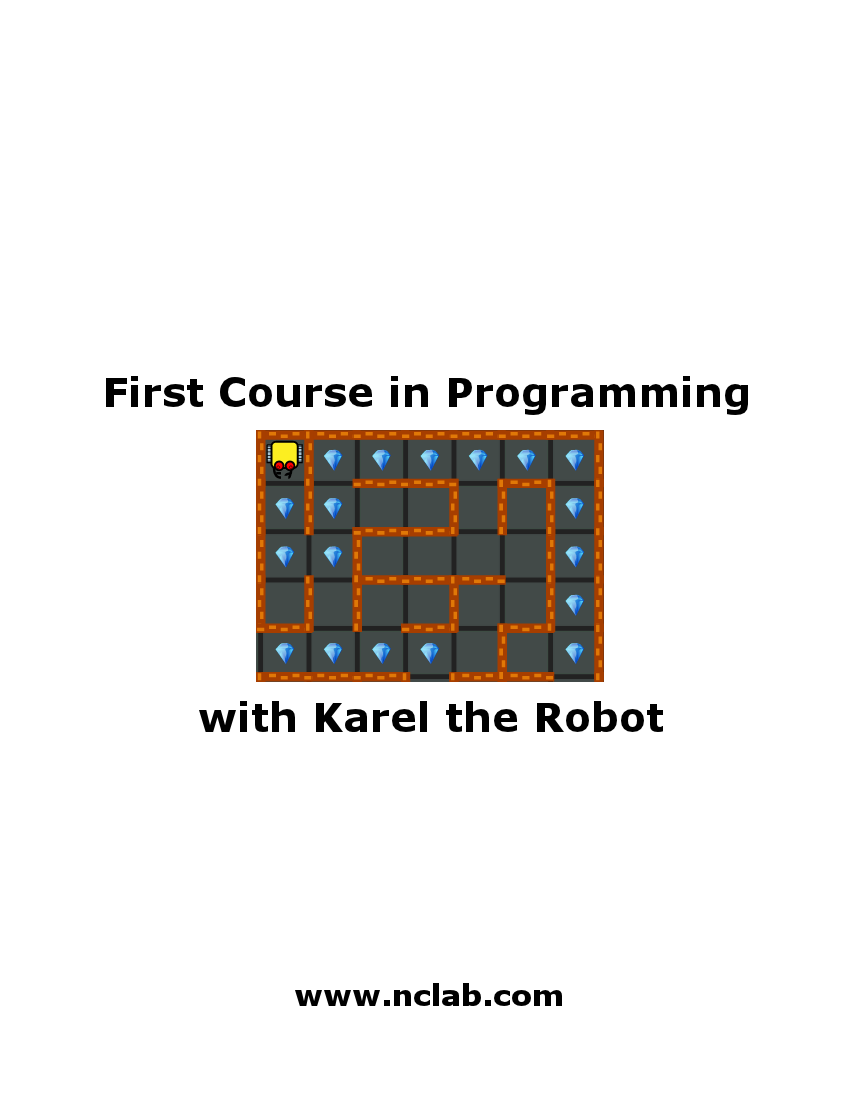
\includegraphics[width=\paperwidth,height=\paperheight]{img/karel-frontpage.png}
%\includegraphics[width=\paperwidth,height=\paperheight]{img/background.jpg}
\vfill
}}}

\begin{document}

% INPUTTING BACKGROUND IMAGE
\AddToShipoutPicture{\BackgroundPic}
\vbox{}
\pagestyle{empty}
\newpage
\textwidth=15.5cm
\ClearShipoutPicture
\newpage

%%%%%%%%%%%%%%%%%%%%%%%%%%%%%%%%%%%%%%%%%%%%%%%%%%%%%%%%%%%%%%%%%%%%%%%%%

\section*{}
\small
\input ../common/aboutnclab.tex

\subsection*{NCLab's Karel vs. the Original Version}
This publication features {\em Karel the Robot}, a programming language 
designed by Richard E. Pattis. Compared to its original version that was
strongly influenced by Pascal, the NCLab version is closer to Python.
There are some other differences as well that make Karel in NCLab easier to use 
for kids -- Karel collects gems instead of beepers, he has a home in the 
maze, and he uses commands that are much easier for kids to understand
and type. For example, {\tt pickbeeper} was replaced with {\tt get}, 
{\tt front-is-clear} was replaced with {\tt wall}, etc. Python 
colons following every command are omitted because using the SHIFT key 
was causing difficulties to some 5 years old programmers. 
Otherwise we have not changed Pattis' original ideas and all functionality 
covered in Pattis' book is available in the Basic Version free of charge. 

\normalsize

\newpage
%{\ }
\setcounter{tocdepth}{2}
\tableofcontents
%\pagestyle{plain}

\newpage

\pagestyle{plain}
\setcounter{page}{1}

%%%%%%%%%%%%%%%%%%%%%%%%%%%%%%%%%%%%%%%%%%%%%%%%%%%%%%%%%%%%%%%%%%%%%%%%%

\section{Introduction}

\subsection{Objectives} 

\begin{itemize}
\item Learn basic facts about the Karel language and its history. 
\item Learn how Karel differs from other programming languages.
\item Learn what this course will help you achieve.
\end{itemize}
This course will teach you principles of modern algorithmic design and  
computer programming with the help of an interactive graphical application 
{\em Karel the Robot} in NCLab. Taking this course will make it much easier 
for you to learn Python, C, C++ and other advanced programming languages. In particular we 
recommend that after Karel you continue with Python, a powerful programming 
language that is used across all science and engineering areas, and yet it is 
technically simpler to handle than C or C++. The textbook
{\em Python Programming for Beginners} is available in PDF via the link 
"Tutorials and Videos" on NCLab home page.

\subsection{Brief history}

Karel the Robot is a famous educational programming language that was introduced by Richard E. 
Pattis in his book "Karel The Robot: A Gentle Introduction to the Art of Programming" in 1981. 
Pattis first used the language in his courses at Stanford University, and now it is used at 
countless schools in the world to introduce students to algorithmic design and computer programming. 
The language is named after Karel \v{C}apek, a Czech writer who invented the word "robot" in his 1921 
science fiction play R.U.R. (Rossum's Universal Robots).

\subsection{Who is Karel?}

Karel is a little robot that lives in a maze, and there are gems in the maze that he loves to collect!
He was manufactured with only five simple commands in his memory:
\begin{itemize}
\item {\color{green} \tt go} ... make one step forward.
\item {\color{green} \tt get} ... pick up a gem from the ground. 
\item {\color{green} \tt left} ... turn to the left.
\item {\color{green} \tt right} ... turn to the right. 
\item {\color{green} \tt put} ... put a gem on the ground. 
\end{itemize}
He also has five built-in sensors that allow him to check his immediate surroundings:
\begin{itemize}
\item {\color{green} \tt wall} ... true if he would crash into a wall by making one more step, false otherwise. 
\item {\color{green} \tt gem} ... true if he stands on a gem, false otherwise.
\item {\color{green} \tt north} ... true if he is facing North, false otherwise.
\item {\color{green} \tt home} ... true if he is at home, false otherwise.
\item {\color{green} \tt empty} ... true if his bag with gems is empty, false otherwise. 
\end{itemize}
During this course you will help Karel solve many exciting tasks starting with very simple ones and 
gradually progressing to more challenging. In this way Karel becomes a great robot, and you 
will become a great programmer!

\subsection{Why should I take this course?}

Computer programming skills are highly valued today, and they will be even more 
valued in the future. Karel's language is so natural that you will be able to 
focus on designing great algorithms. This is the most important skill in 
computer programming. In other words, you could start learning programming 
with a technically 
complicated conventional programming language as well, but you would spend lots of time 
battling technical problems. The advantage of starting with Karel is that 
when moving on to other languages, you will be able to focus on the technical 
differences, as the programming concepts you will already understand.


\subsection{Is Karel a toy language?}

Definitely not! Despite its playful appearance, Karel contains all elements 
of modern procedural programming. The complexity of algorithms 
that you will encounter in this course ranges from {\em extremely simple} 
to {\em extremely tough}. Towards the end of this course you will encounter 
tasks that will make your head spin. However, Karel is very light on 
technicalities, which is very good for someone who is just starting out.

The biggest conceptual difference between Karel and standard procedural
programming languages such as Python, C, C++ or Fortran is that {\em the robot does not 
know math}. At least not until we get to advanced levels that are beyond 
the original Pattis' book. In the basic course, you will solve many exercises 
whose objective is to teach you how to design great algorithms, and math is 
not needed for that. After finishing this tutorial, you will be able to transition 
smoothly to Python where you can do as much math as you like!
 
\subsection{Review questions}

All review questions in this textbook are multiple-choice. One or more 
answers may be correct.

\begin{enumerate}
\item Name the university where Karel the Robot was created:
\begin{enumerate}
\item[A1] MIT
\item[A2] Princeton
\item[A3] Harvard
\item[A4] Stanford
\end{enumerate}
\item What is the programming language that you should learn after Karel?
\begin{enumerate}
\item[A1] C
\item[A2] Python
\item[A3] Haskell
\item[A4] Fortran
\end{enumerate}
\item What is the biggest conceptual difference between Karel and standard
      procedural programming languages such as Python, C, C++ or Fortran?
\begin{enumerate}
\item[A1] Karel only knows five commands.
\item[A2] Karel only can do simple algorithms.
\item[A3] Karel does not know math.
\item[A4] Karel has only five sensors.
\end{enumerate}
\item Where does Karel live and what objects does he like to collect?
\begin{enumerate}
\item[A1] Karel lives in a maze and he likes to collect gems.
\item[A2] Karel lives in a cave and he likes to collect gold nuggets.
\item[A3] Karel lives on an island and he likes to collect coconuts.
\item[A4] Karel lives in a marketplace and he likes to collect coins from the ground.
\end{enumerate}
\item What is the command that moves the robot one step forward?
\begin{enumerate}
\item[A1] step
\item[A2] forward
\item[A3] go
\item[A4] move
\end{enumerate}
\item What is the command that turns the robot to the left?
\begin{enumerate}
\item[A1] left\_turn
\item[A2] turn\_left
\item[A3] turnleft
\item[A4] left
\end{enumerate}
\item What is the command that turns the robot to the right?
\begin{enumerate}
\item[A1] right\_turn
\item[A2] right
\item[A3] turnright
\item[A4] turn\_right
\end{enumerate}
\item What is the command to pick up a gem from the ground?
\begin{enumerate}
\item[A1] pick
\item[A2] pick\_gem
\item[A3] get
\item[A4] get\_gem
\end{enumerate}
\item What is the command to drop a gem on the ground?
\begin{enumerate}
\item[A1] put
\item[A2] drop\_gem
\item[A3] drop 
\item[A4] put\_gem
\end{enumerate}
\item What sensor helps the robot avoid crashing into walls?
\begin{enumerate}
\item[A1] wall\_ahead
\item[A2] wall
\item[A3] crash
\item[A4] danger
\end{enumerate}
\item What sensor helps the robot detect gems?
\begin{enumerate}
\item[A1] detect\_gem
\item[A2] see\_gem
\item[A3] gem
\item[A4] near\_gem
\end{enumerate}
\item What sensor does the robot use to check whether he has any gems in his bag?
\begin{enumerate}
\item[A1] bag\_full
\item[A2] bag\_empty
\item[A3] has\_gems
\item[A4] empty
\end{enumerate}
\item What sensor helps the robot detect his orientation?
\begin{enumerate}
\item[A1] south
\item[A2] north
\item[A3] east
\item[A4] west
\end{enumerate}
\item What sensor helps the robot detect whether he is at home?
\begin{enumerate}
\item[A1] at\_home
\item[A2] finished
\item[A3] home
\item[A4] stop
\end{enumerate}
\item What is the most important skill in computer programming?
\begin{enumerate}
\item[A1] Writing short programs.
\item[A2] Designing great algorithms.
\item[A3] Writing programs quickly.
\item[A4] Knowing many programming languages.
\end{enumerate}
\end{enumerate}

\section{Exploring NCLab}

\subsection{Objectives} 

\begin{itemize}
\item Get acquainted with NCLab.
\end{itemize}
Before beginning this course, we invite you to create an account in 
NCLab, log in, and take a while to explore the many activities 
that NCLab offers. A great companion reading is {\em Intro to NCLab - Part I 
(Meet the Cloud)} that is available in PDF via the link "Tutorials and Videos"
on NCLab home page {\tt http://nclab.com}.

\subsection{Review questions}

Review questions for this Section are located in the document {\em Intro to NCLab - Part I 
(Meet the Cloud)}.

\section{Launching Karel}

\subsection{Objectives} 
\begin{itemize}
\item Learn to launch Karel and work with the graphical application.
\item Learn to clone displayed projects.
\item Learn that karel has several modes.
\end{itemize}
Karel can be launched in several different ways. The simplest one is to click on the icon 
{\em Programming} and select {\em Karel} in the menu. This will launch the application 
with a randomly generated maze, as shown in Fig. \ref{fig:init}.


\begin{figure}[!ht]
\begin{center}
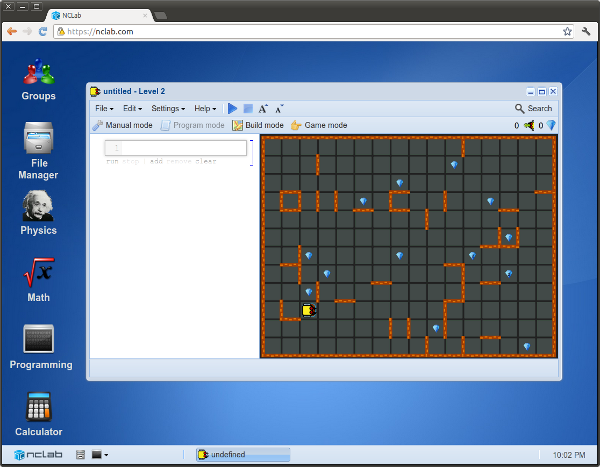
\includegraphics[width=0.9\textwidth]{img/init.png}
\end{center}
\vspace{-2mm}
\caption{Launching Karel via the Programming icon.}
\label{fig:init}
\vspace{-1cm}
\end{figure}
\newpage
\noindent
Karel will be launched in {\em Programming mode} which is the most-frequently 
used one. You can easily switch to the {\em Manual mode}, {\em Builder},
and {\em Game mode} in the menu. Game mode is available in Full Version only. 
These modes will be discussed in Paragraph \ref{levels}.

\subsection{Karel's window} \label{menu}

The application window contains two lines of menus and information on top,
work area on the left, maze on the right, and status bar on the bottom.
The menus are fairly intuitive, so let us just explain a few selected functions, starting 
with the {\em File} menu:

{\em Open} will open a file from your NCLab account (not from your hard disk). {\em New} will generate a new random maze.
{\em Clone} will copy a Displayed Project into your account (to be discussed in Paragraph \ref{cloning}). 
{\em Display} will submit your project for review. If you think that 
      other users would find your program or game interesting, this is the way to make it 
      available to them. Upon passing the review, your project will be added to Displayed Projects.

{\em Edit} menu allows you to operate with input and text cells (to be discussed in 
Section \ref{sec:editmenu}). In {\em Settings} you can change Karel's {\em Level} (to be discussed
in Paragraph \ref{levels}), change his speed, and adjust sound preferences. The blue arrow and square 
buttons are used to run and stop programs, and the two buttons next to them can be used to increase and decrease 
font size. The pair of icons on far right is the step counter (that can be reset by clicking on it) and 
gem counter that indicates how many gems Karel has in his bag.

\subsection{Cloning Displayed Projects} \label{cloning}

All programs and exercises that we will work with are
available for you to clone. To do this, 
click on the File Manager icon. In the File Manager's menu go to 
{\em Project} and then click on {\em Clone}. This will launch a new window 
with Displayed Projects as shown in Fig. \ref{fig:cloning}.

\newpage
\begin{figure}[!ht]
\begin{center}
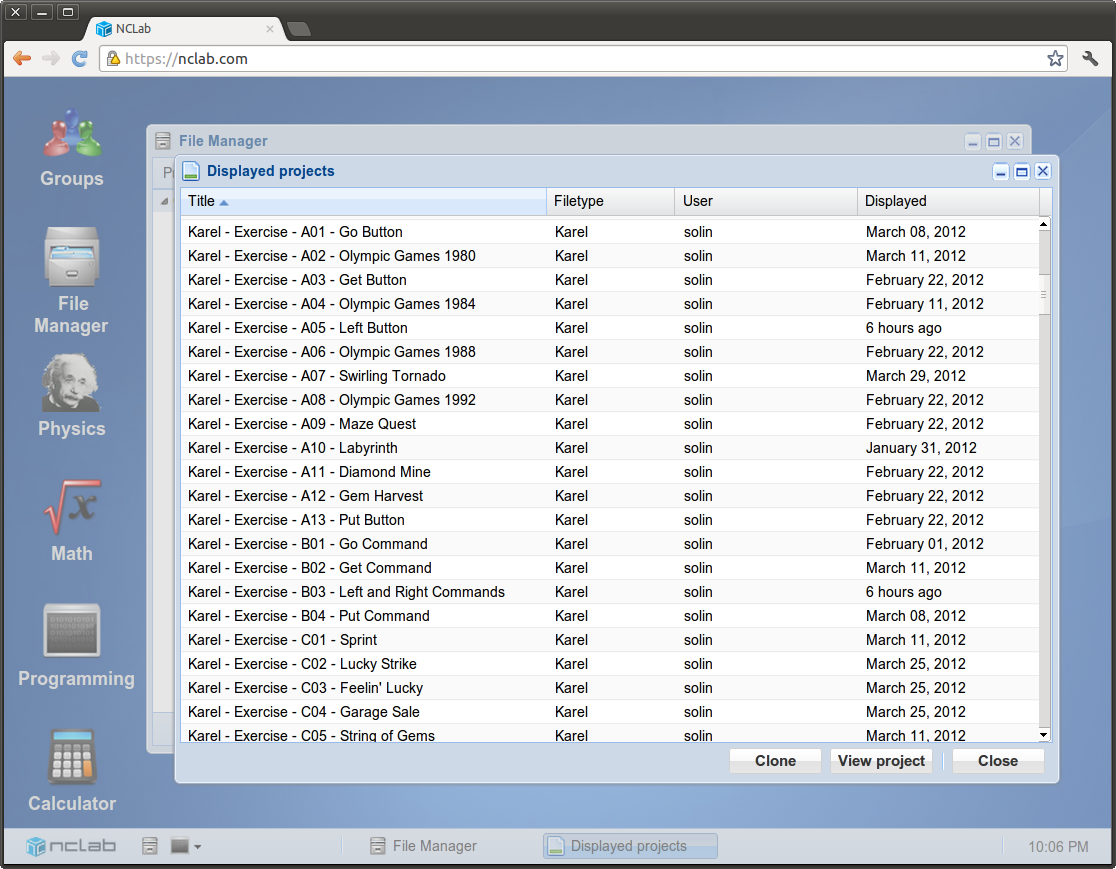
\includegraphics[width=0.9\textwidth]{img/cloning.png}
\end{center}
%\vspace{-2mm}
\caption{File Manager's {\em Project} menu allows you to clone many Karel projects.}
\label{fig:cloning}
\end{figure}
\noindent
All projects whose names start with "Karel - Exercise" are of particular interest 
for this tutorial. Their solutions have names starting with "Karel - Solution". 
Any of them can be cloned into your account via clicking on the project name in the window, 
and pressing the button {\em Clone}.

In the File Manager's right-hand side panel, you will see the list of all 
projects that you cloned. Click on any of them to launch it. You are free to 
use the cloned projects as they are, or modify them in any way you like. Your 
modifications will not affect the original. And, you can 
always synchronize your version with the original, via 
a right-click on the project in the File Manager and selecting {\em Synchronize}.
Keep in mind though -- synchronizing with the original will erase any changes that 
you made to the project.

%\subsection{Basic and Full Versions}
%
%Users sponsored by an institution are using NCLab in Full Version. Some limitations 
%apply to users who use NCLab in Basic Version (see Terms of Use for details). These 
%users have an Upgrade icon on their Desktop, that they can use to upgrade 
%NCLab to Full Version for a symbolic monthly subscription fee.

\subsection{Karel modes} \label{levels}

Karel operates in four modes:
\begin{itemize}
\item {\em Manual mode:} The robot is controlled using the mouse and five buttons Go, Get, Left, Right, and Put. 
      Watch out and do not crash!
\item {\em Program mode:} The robot is controlled using written programs (computer code). The Program mode is 
      split into several Levels:
\begin{itemize}
\item Level 1 is a transition layer between the Manual and Programming modes. Programs are written using only 
      five commands {\tt go}, {\tt get}, {\tt left}, {\tt right}, and {\tt put} that exactly correspond to 
      the buttons Go, Get, Left, Right, and Put in Manual mode.
\item Level 2 is where the actual programming begins. On top of the commands from Level 1, programs can contain 
      conditions, loops, and custom commands.
\item Level 3 teaches the user to operate with logical and numerical variables, and with computer memory. Karel  
      also has receives a GPS device. This Level is in preparation.
\item Level 4 teaches the basics of object-oriented programming. This Level is in preparation.
\item Level 5 teaches the basics of parallel programming. This Level is in preparation.
\end{itemize}
\item {\em Build mode:} This mode allows the user to create custom mazes.
\item {\em Game mode:} Makes it possible to create and play games. 
\end{itemize}

\subsection{Review questions}

\begin{enumerate}
\item What can you do with a displayed Karel project that you clone into your account?.
\begin{enumerate}
\item[A1] View but not run.
\item[A2] View and run but not edit.
\item[A3] View, run and edit but not save.
\item[A4] View, run, edit, save, whatever, they are all yours!
\end{enumerate}
\item What are the four modes of the Karel application?
\begin{enumerate}
\item[A1] Manual mode, Build mode, Program mode, Game mode.
\item[A2] Mode 1, Mode 2, Mode 3, Mode 4.
\item[A3] Beginner mode, Intermediate mode, Advanced mode, Expert mode.
\item[A4] Karel has no modes.
\end{enumerate}
\item What is the difference between Levels 1 and 2?
\begin{enumerate}
\item[A1] In Level 2 the robot has more sensors. 
\item[A2] In Level 2 one can only guide the robot with the mouse.
\item[A3] In Level 2 one can only use 5 commands.
\item[A4] In Level 2 programs can contain 
      conditions, loops, and custom commands.
\end{enumerate}
\end{enumerate}


\section{Section A - Operating the Robot in Manual Mode}

\subsection{Objectives} 
\begin{itemize}
\item Learn to operate the robot in Manual mode using five buttons Left, Right, Go, Get and Put.
\end{itemize}
There are thirteen exercises A01 - A13 for you to solve.
Each exercise can be cloned via the File Manager's 
{\em Project} menu as described in Paragraph \ref{cloning}. 
Do not skip levels since each one has something new! 

\newpage
\subsection{Exercise A01 - Go Button}

{\em Karel is returning from a long walk and his batteries are running out. 
Use the buttons on the left to get him home quickly! }

\begin{figure}[!ht]
\begin{center}
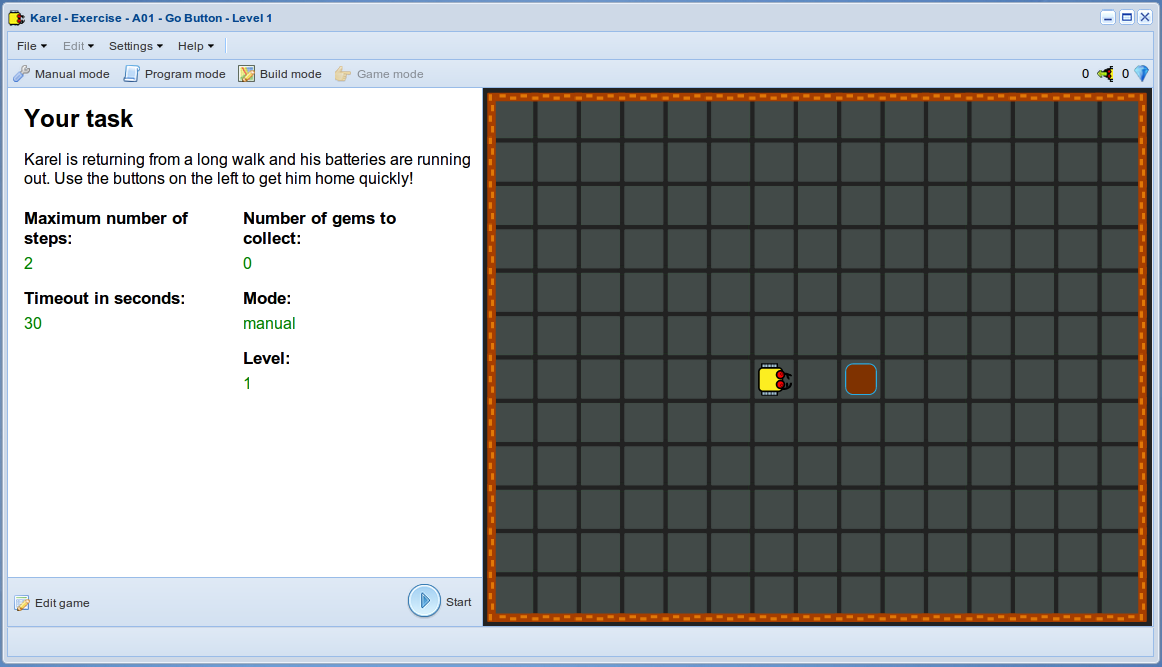
\includegraphics[width=0.7\textwidth]{img/a01.png}
\end{center}
\vspace{-4mm}
\caption{In the first exercise you need to help the robot get home.}
\label{fig:a01}
\end{figure}
\noindent
Pressing Start will start 
the exercise, and at this time also the buttons Go, Left, Right, Put and Get appear, 
as shown in Fig. \ref{fig:a01b}.


\begin{figure}[!ht]
\begin{center}
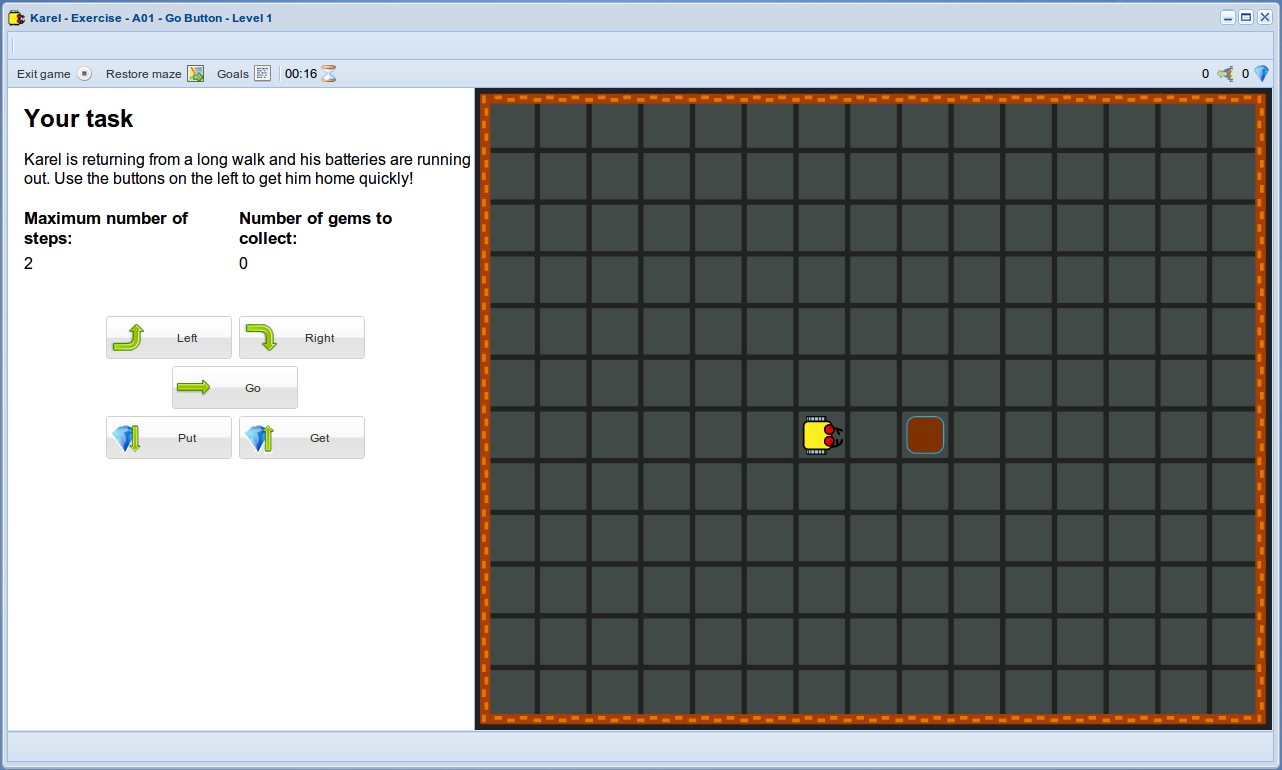
\includegraphics[width=0.7\textwidth]{img/a01b.png}
\end{center}
\vspace{-4mm}
\caption{Karel can be guided manually, using five buttons located in the left panel.}
\label{fig:a01b}
\end{figure}


\subsection{Exercise A02 - Olympic Games 1980}

{\em Karel is training for Robolympic Games! Your task is to run with 
the robot home as fast as possible. Karel's personal record is four seconds. How fast can you be?}

\begin{figure}[!ht]
\begin{center}
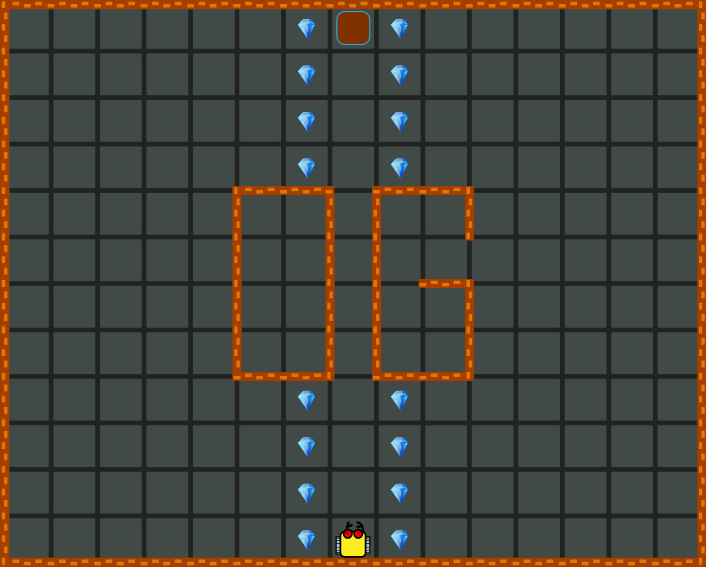
\includegraphics[width=0.7\textwidth]{img/a02.png}
\end{center}
\vspace{-4mm}
\caption{Karel is training for Robolympic Games.}
\label{fig:a02}
\vspace{-4mm}
\end{figure}
\noindent

\subsection{Exercise A03 - Get Button}

{\em Today is Karel's lucky day because he is about to find his first gem. 
Use the buttons on the left to help the robot pick up the gem and carry it 
home!}

\begin{figure}[!ht]
\begin{center}
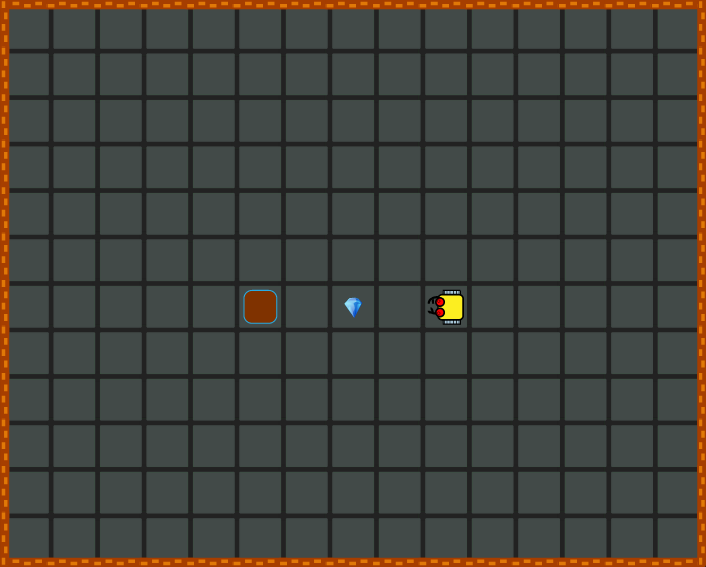
\includegraphics[width=0.7\textwidth]{img/a03.png}
\end{center}
\vspace{-4mm}
\caption{Karel is about to find his first gem.}
\label{fig:a03}
\vspace{-1cm}
\end{figure}
\noindent

\newpage
\subsection{Exercise A04 - Olympic Games 1984}

{\em It is Robolympic season again! Run home as fast as you can, 
and collect all three gems on the way! Karel's personal record is 10 seconds.}


\begin{figure}[!ht]
\begin{center}
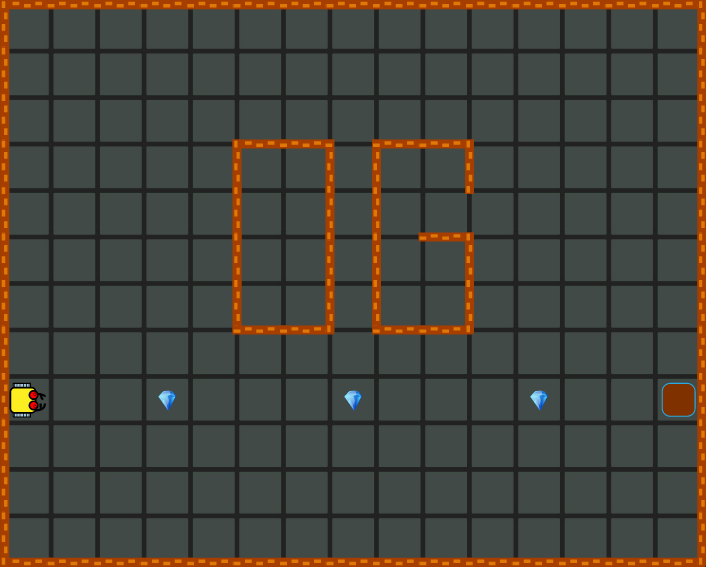
\includegraphics[width=0.7\textwidth]{img/a04.png}
\end{center}
\vspace{-4mm}
\caption{Karel's second Robolympic Games.}
\label{fig:a04}
\vspace{-1cm}
\end{figure}
\noindent


\subsection{Exercise A05 - Left Button}

{\em Help the robot collect the gem and return home!}

\begin{figure}[!ht]
\begin{center}
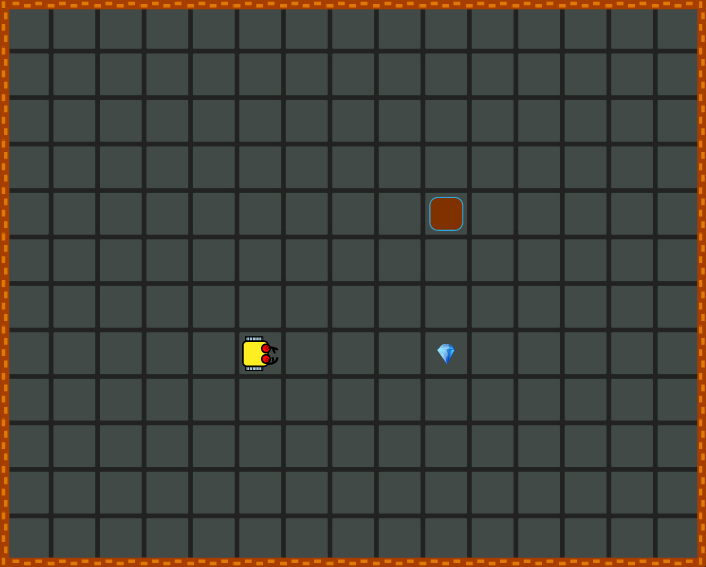
\includegraphics[width=0.7\textwidth]{img/a05.png}
\end{center}
\vspace{-4mm}
\caption{Karel is about to learn how to make a left turn.}
\label{fig:a05}
\vspace{-1cm}
\end{figure}
\noindent

\newpage

\subsection{Exercise A06 - Olympic Games 1988 }

{\em Karel is training for his third Robolympic Games. Run with him around the block and home as fast as possible. He needs to collect at least one gem on the way. Karel's personal record is 16 seconds!}

\begin{figure}[!ht]
\begin{center}
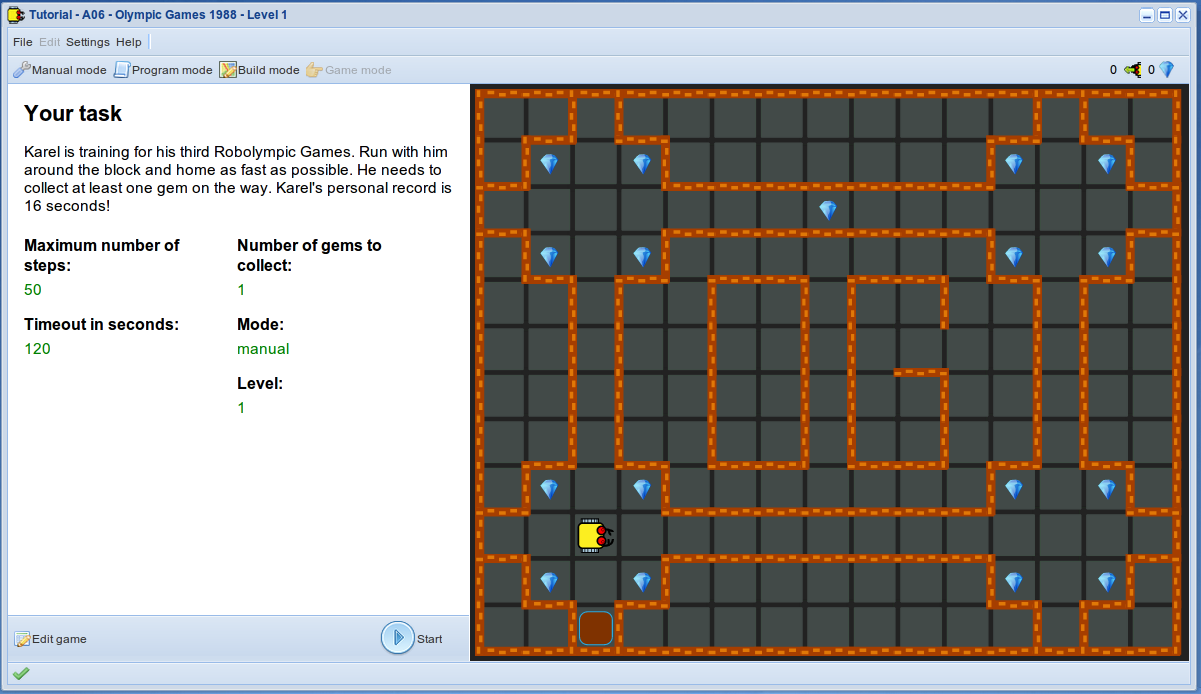
\includegraphics[width=0.7\textwidth]{img/a06.png}
\end{center}
\vspace{-4mm}
\caption{Karel's third Robolympic Games.}
\label{fig:a06}
\vspace{-1cm}
\end{figure}
\noindent


\subsection{Exercise A07 - Right Button}

{\em Pick up the two gems and get Karel home!}

\begin{figure}[!ht]
\begin{center}
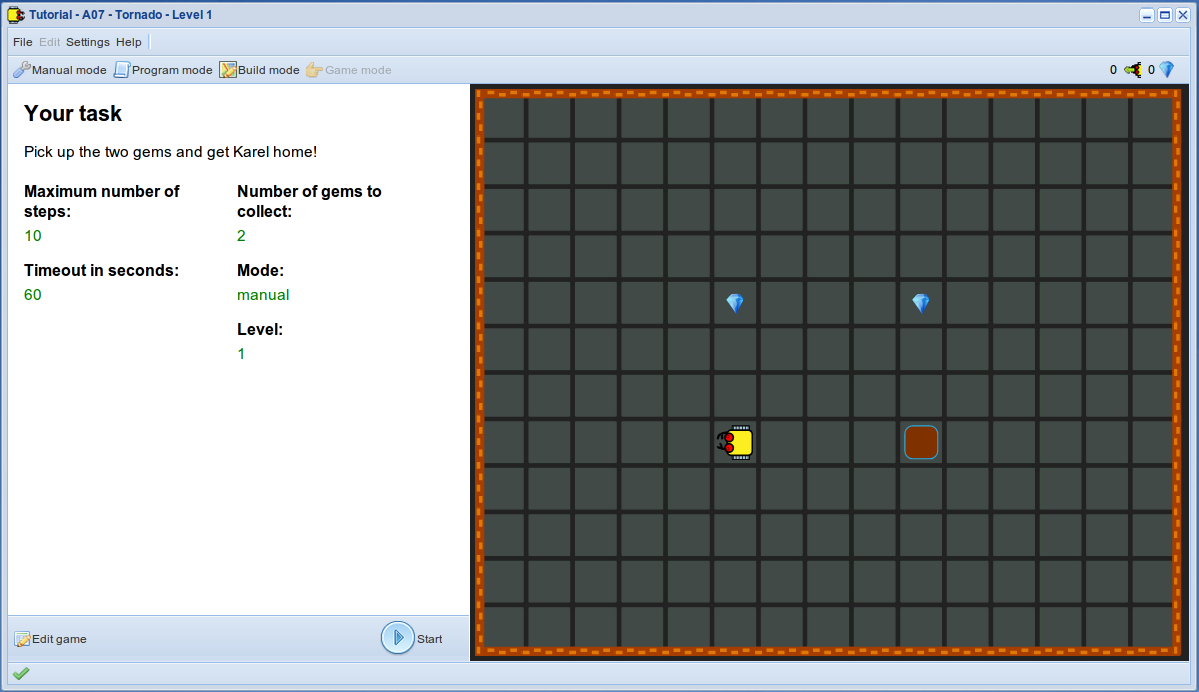
\includegraphics[width=0.7\textwidth]{img/a07.png}
\end{center}
\vspace{-4mm}
\caption{Karel needs to collect two gems and get home.}
\label{fig:a07}
\vspace{-1cm}
\end{figure}
\noindent
\newpage

\subsection{Exercise A08 - Olympic Games 1992}

{\em Last season of Karel's Robolympics Games is here! The 
robot needs to run home as fast as possible and bring one gem. 
Be careful not to crash, this is a tricky level! Karel's personal record is 26 seconds.}\\[-7mm]

\begin{figure}[!ht]
\begin{center}
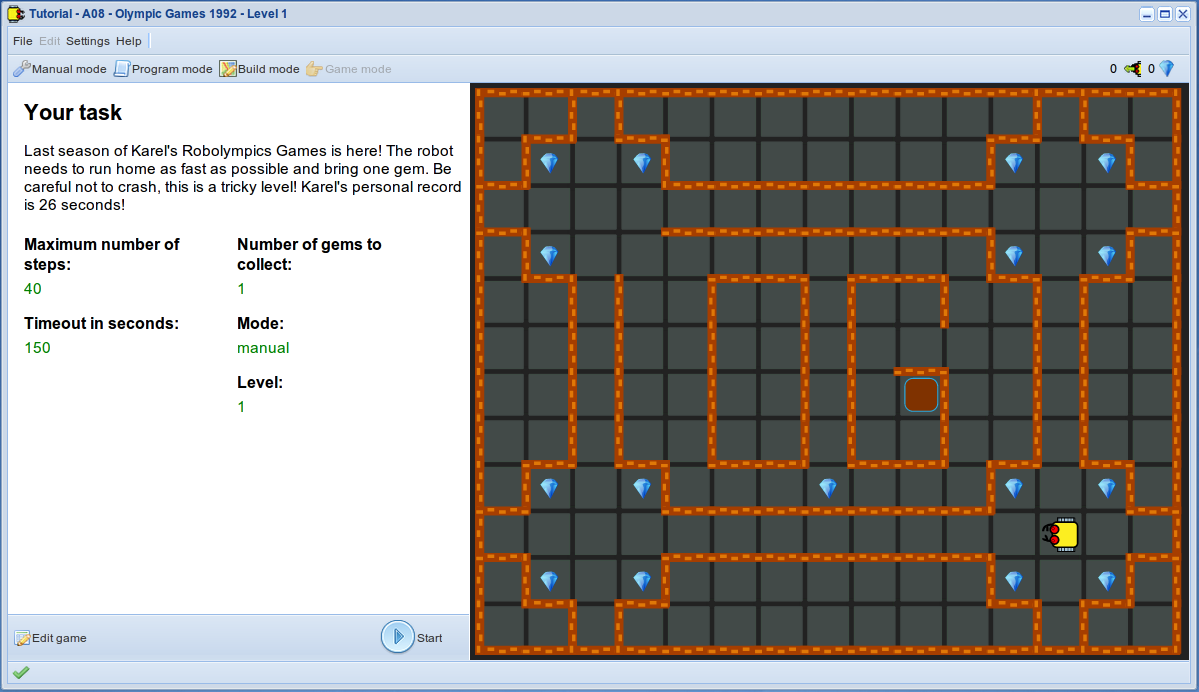
\includegraphics[width=0.7\textwidth]{img/a08.png}
\end{center}
\vspace{-4mm}
\caption{Karel's fourth Robolympic Games.}
\label{fig:a08}
\vspace{-4mm}
\end{figure}
\noindent

\subsection{Exercise A09 - Maze Quest}

{\em This time Karel got seriously lost while looking for his favorite gem. 
Help him to collect the gem and find his way home!}\\[-7mm]

\begin{figure}[!ht]
\begin{center}
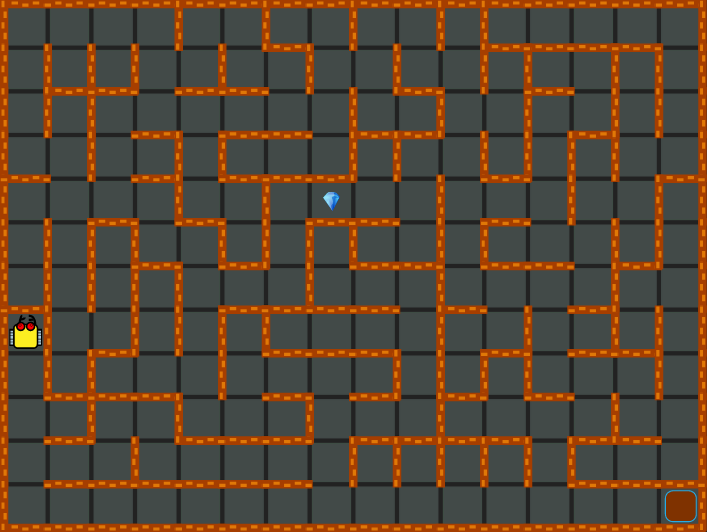
\includegraphics[width=0.7\textwidth]{img/a09.png}
\end{center}
\vspace{-4mm}
\caption{Karel got lost while looking for his favorite gem.}
\label{fig:a09}
\vspace{-4mm}
\end{figure}
\noindent
\newpage

\subsection{Exercise A10 - Labyrinth}

{\em This is a true labyrinth and your task is to lead Karel 
home. Remember - think first before going anywhere!}

\begin{figure}[!ht]
\begin{center}
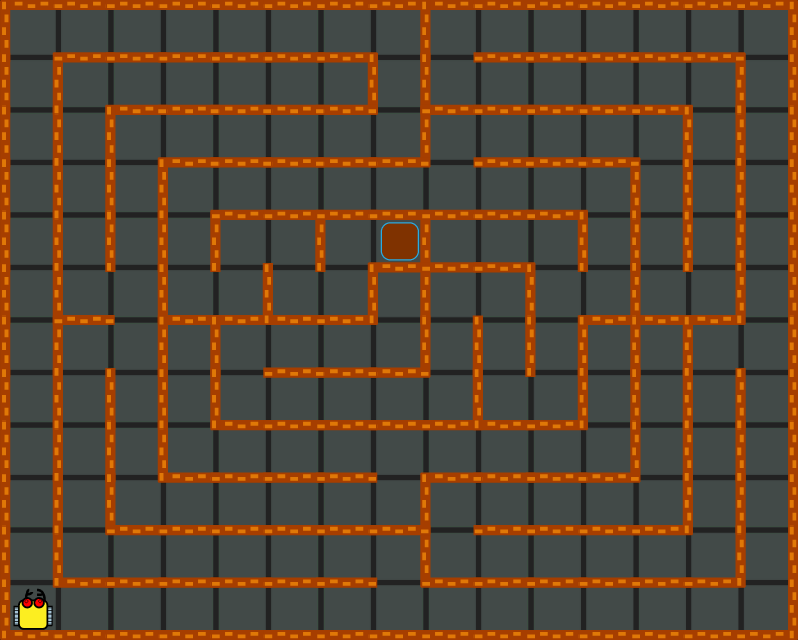
\includegraphics[width=0.7\textwidth]{img/a10.png}
\end{center}
\vspace{-4mm}
\caption{Karel needs to find his way home in a labyrinth.}
\label{fig:a10}
\vspace{-4mm}
\end{figure}
\noindent


\subsection{Exercise A11 - Diamond Mine}

{\em Karel discovered an abandoned diamond mine. Use the buttons
on the left to collect all gems and get back home in time!}

\begin{figure}[!ht]
\begin{center}
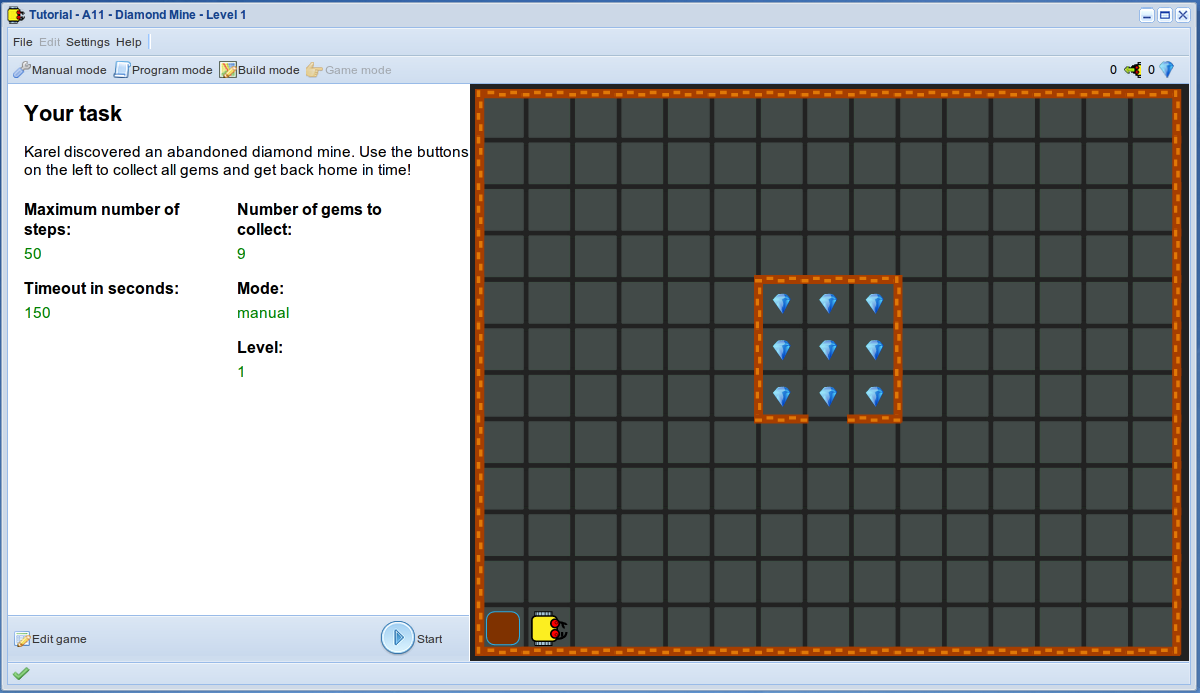
\includegraphics[width=0.7\textwidth]{img/a11.png}
\end{center}
\vspace{-4mm}
\caption{Karel found an abandoned diamond mine.}
\label{fig:a11}
\vspace{-4mm}
\end{figure}
\noindent
\newpage

\subsection{Exercise A12 - Gem Harvest}

{\em If gems are piled up, then a number is showing their amount. 
Help Karel collect all gems in this maze and return home!}\\[-7mm]

\begin{figure}[!ht]
\begin{center}
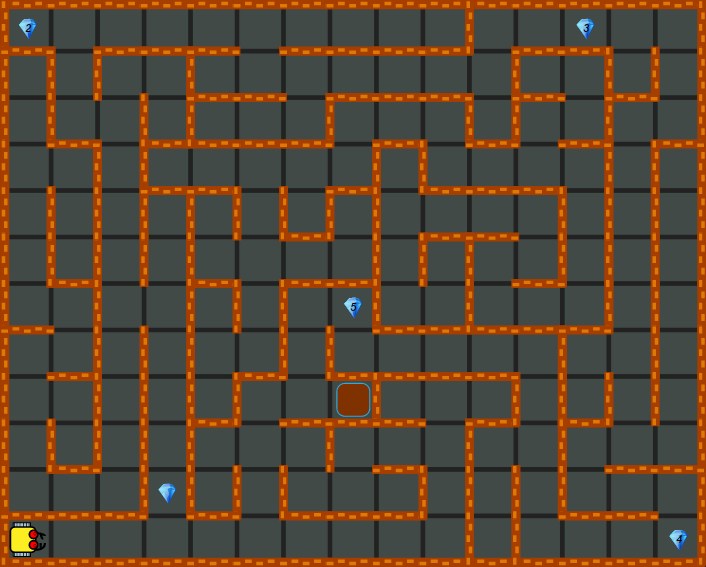
\includegraphics[width=0.7\textwidth]{img/a12.png}
\end{center}
\vspace{-4mm}
\caption{If gems are piled up, then a number is showing their amount.}
\label{fig:a12}
\vspace{-4mm}
\end{figure}
\noindent


\subsection{Exercise A13 - Put Button}

{\em Karel has five gems in his bag. Use the buttons on the left to put the gems on the table and 
return home in time!}\\[-7mm]

\begin{figure}[!ht]
\begin{center}
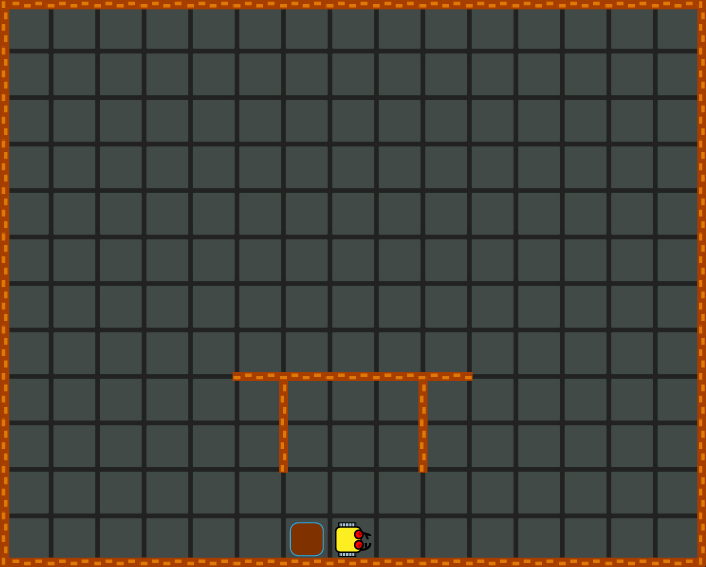
\includegraphics[width=0.7\textwidth]{img/a13.png}
\end{center}
\vspace{-4mm}
\caption{Karel needs to put five gems on the table.}
\label{fig:a13}
\vspace{-4mm}
\end{figure}
\noindent
\newpage

\section{Section B - Bridge to Programming}

\subsection{Objectives} 
 
\begin{itemize}
\item Start operating the robot in Programming mode using simple instructions.
\end{itemize}
In Programming mode, the robot obeys written commands 
{\tt left}, {\tt right}, {\tt go}, {\tt get}, and {\tt put}.
These commands have exactly the same function as the corresponding buttons in Manual mode.
You can clone all exercises in this Section into your account via the File Manager's {\em Project}
menu, same as you did with the ones in Section A.

\subsection{Review questions}

\begin{enumerate}
\item What command moves the robot one step forward?
\begin{enumerate}
\item[A1] forward
\item[A2] step
\item[A3] go
\item[A4] move
\end{enumerate}
\item What command turns the robot to the left?
\begin{enumerate}
\item[A1] left
\item[A2] turnleft
\item[A3] left\_turn
\item[A4] turn\_left
\end{enumerate}
\item What command turns the robot to the right?
\begin{enumerate}
\item[A1] right\_turn
\item[A2] right
\item[A3] turnright
\item[A4] turn\_right
\end{enumerate}
\item What command tells Karel to pick up a gem from the ground?
\begin{enumerate}
\item[A1] pick
\item[A2] pick\_gem
\item[A3] get
\item[A4] get\_gem
\end{enumerate}
\item What command tells the robot to drop a gem on the ground?
\begin{enumerate}
\item[A1] put
\item[A2] drop\_gem
\item[A3] drop 
\item[A4] put\_gem
\end{enumerate}
\end{enumerate}

\newpage
\subsection{Exercise B01 - Go Command}

{\em Write a program that gets Karel home! Remember: Always write one command per line.}

\begin{figure}[!ht]
\begin{center}
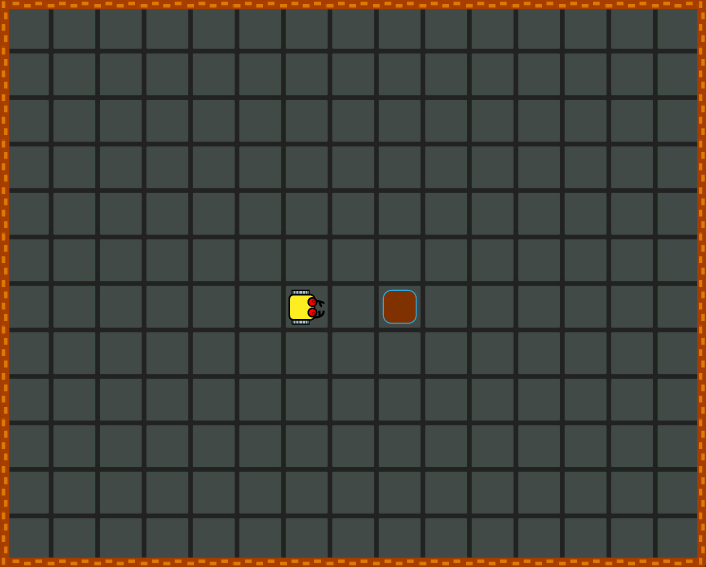
\includegraphics[width=0.7\textwidth]{img/b01.png}
\end{center}
\vspace{-4mm}
\caption{Get Karel home using the {\tt go} command.}
\label{fig:b01}
\vspace{-4mm}
\end{figure}
\noindent

\subsection{Exercise B02 - Get Command}

{\em Write a program for Karel to collect all gems and get home! 

\begin{figure}[!ht]
\begin{center}
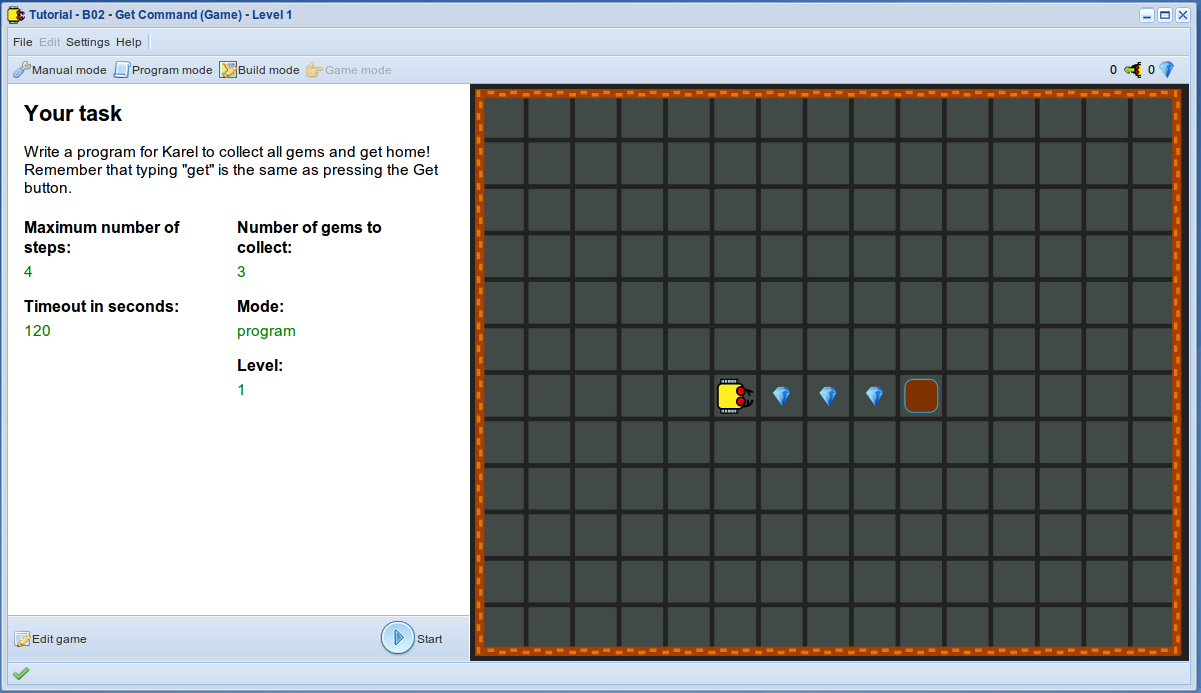
\includegraphics[width=0.7\textwidth]{img/b02.png}
\end{center}
\vspace{-4mm}
\caption{Collecting gems via the {\tt get} command.}
\label{fig:b02}
\vspace{-4mm}
\end{figure}
\noindent

\newpage

\subsection{Exercise B03 - Left and Right Commands}

{\em Write a program for Karel to collect the gem and return home! 

\begin{figure}[!ht]
\begin{center}
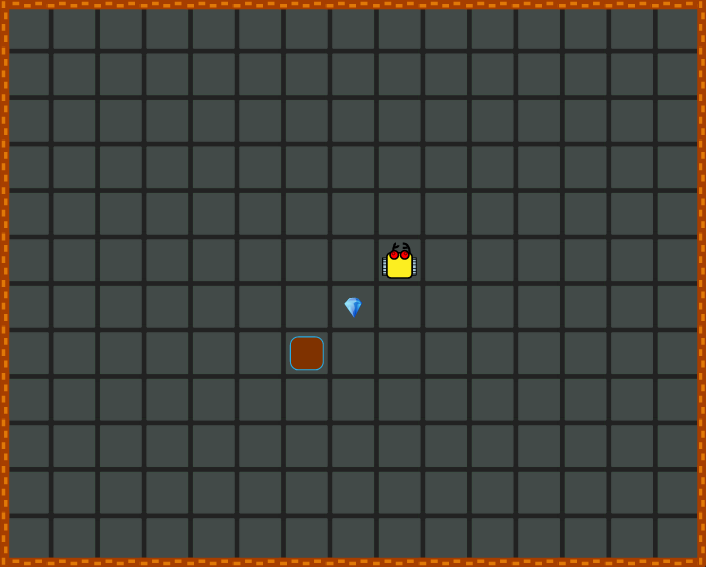
\includegraphics[width=0.7\textwidth]{img/b03.png}
\end{center}
\vspace{-4mm}
\caption{Turning to the left and to the right via the {\tt left} and {\tt right} commands.}
\label{fig:b03}
\vspace{-4mm}
\end{figure}
\noindent

\subsection{Exercise B04 - Put Command}

{\em Write a program for Karel to pick up the gem, turn around, make 
two steps, put the gem on the ground, and return home!}



\begin{figure}[!ht]
\begin{center}
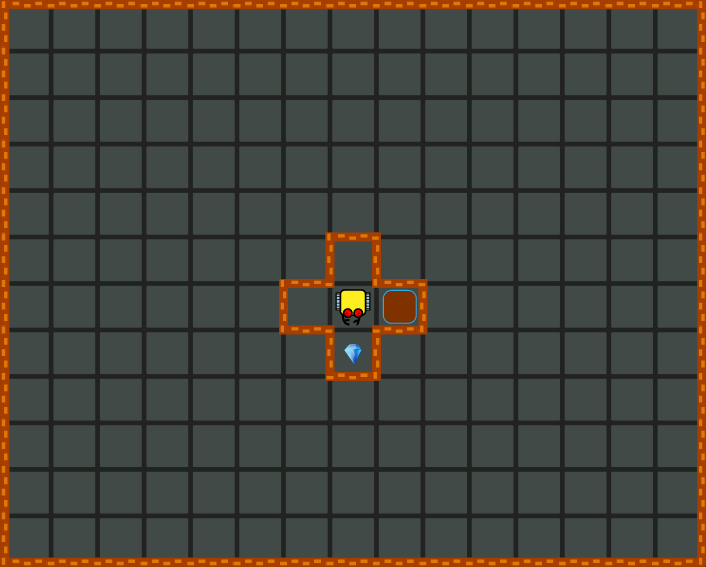
\includegraphics[width=0.7\textwidth]{img/b04.png}
\end{center}
\vspace{-4mm}
\caption{Karel moves a gem from one corner to another using the {\tt put} command.}
\label{fig:b04}
\vspace{-4mm}
\end{figure}
\noindent
\newpage

\section{Intermission - Algorithms, Programs, and Bugs}

\subsection{Objectives} 
 
\begin{itemize}
\item Understand the difference between {\em algorithm} and {\em program}. 
\item Learn the difference between {\em syntactical} and {\em logical} mistakes.
\item Understand that {\em debugging} is an indivisible part of computer programming.
\end{itemize}
Karel always obeys all commands {\em precisely}. Sometimes it may happen that 
we plan one thing but to our surprise the robot does something else. In most cases this 
happens when our {\em algorithm} is wrong. By an {\em algorithm} we mean a sequence of 
logical steps that the robot needs to follow in order to fulfill his task. Algorithms 
are presented using normal human language, not in terms of the robot's commands. 

{\em Program} or {\em computer code} is created when the algorithm is expressed
in terms of the robot's language. When our algorithm is good, then 
the program is easy to write.

Mistakes in algorithms are called {\em logical errors}. A logical error is, for 
example, when we crash the robot into a wall because we forgot to make a turn.
Mistakes such as mis-spelling a command or forgetting indentation are related to 
the {\em syntax} and they are called {\em syntactical errors}. Of these two types, 
logical errors are usually much more difficult to find. 

In general, mistakes or either kind are called {\em bugs} and the procedure of 
eliminating them is called {\em debugging}. Depending on how careful we 
were while preparing our algorithm and writing the program, debugging takes either 
a short time or a long time. It does not happen often that a program works correctly
right away. 

When we commit a syntactical error (such as mis-spelling a command)
the robot will write an error message without doing anything else.
If our algorithm contains a logical error based on which the robot crashes 
into a wall, if we ask him to collect a gem where there is none, or if we 
ask him to put a gem on the ground while his bag is empty, then he will
write an error message and stop executing the program. 

\subsection{Review questions} 

\begin{enumerate}
\item What is an {\em algorithm}?
\begin{enumerate}
\item[A1] Very short program.
\item[A2] Sequence of instructions for the robot written using the correct commands.
\item[A3] Logical mistake in our program.
\item[A4] Sequence of logical steps leading to the solution of the given task.
\end{enumerate}
\item What is a {\em program}?
\begin{enumerate}
\item[A1] Sequence of logical steps written using human language.
\item[A2] Algorithm that does not contain any mistakes.
\item[A3] Algorithm that is translated from human language to the robot's language.
\item[A4] Very long algorithm.
\end{enumerate}
\item If the robot does something unexpected, what is the most probable reason for that?
\begin{enumerate}
\item[A1] Something is wrong with the computer.
\item[A2] Internet connection is too slow.
\item[A3] Web browser needs upgrading.
\item[A4] Our algorithm contains a logical mistake.
\end{enumerate}
\item What of the following is a {\em logical} mistake?
\begin{enumerate}
\item[A1] Mistake in an algorithm that causes the robot to do something unexpected.
\item[A2] Opening Karel through the Programming menu instead of through File Manager. 
\item[A3] Typing a command in a wrong way, such as {\tt lft} instead of {\tt left}.
\item[A4] Learning Fortran.
\end{enumerate}
\item What of the following is a {\em syntactical} mistake?
\begin{enumerate}
\item[A1] Writing two commands on the same line.
\item[A2] Having two empty characters between commands.
\item[A3] Mis-spelling a command.  
\item[A4] Mistake that causes the robot to do something unexpected.
\end{enumerate}
\item What do we mean by {\em debuging}?
\begin{enumerate}
\item[A1] Apologizing after we ask a friend too many questions.
\item[A2] Playing an algorithm in our head prior to writing a program. 
\item[A3] Looking for mistakes when our program does not work.
\item[A4] Writing a new program after the previous one did not work.
\end{enumerate}
\end{enumerate}

\section{Section C - Counting Loop}

\subsection{Objectives} 

\begin{itemize}
\item Learn to make the robot repeat something a given number of times.
\end{itemize}

\noindent
In Section B we successfully crossed the bridge between manual control 
and programming. The bridge collapsed, there is no way back. But do 
not worry about that, the land of Programming is much more beautiful!


\subsection{The {\tt repeat} command}

The counting loop, represented by the {\tt repeat} command, can save 
us lots of writing when something is repeated. For example, for 
Karel to make seven steps forward we could type:

\begin{verbatim}
go
go
go
go
go
go
go
\end{verbatim}
But this is neither efficient nor elegant. Instead, the same can be
achieved by telling Karel to {\tt repeat} the {\tt go} command {\tt 7} times:

\begin{verbatim}
repeat 7
  go
\end{verbatim}
There are a few simple rules that we need to remember when using the {\tt repeat} command:

\begin{itemize}
\item Keep code readable -- always write one command per line.
\item Indentation -- all commands to be repeated (the {\em body of the loop}) need to be indented. You can
      choose whether you prefer 2-indents or 4-indents. The former yields more compact 
      code with not-so-long lines, the latter is easier to read. 
\item Cancel the indentation for the first command that does not belong to the body of the loop.
\end{itemize}
To illustrate what the indentation does, let's look at a code that will move the robot 8 steps forward:

\begin{verbatim}
repeat 4
  go
  go
\end{verbatim}
Compare to a code that will only move the robot 5 steps forward:

\begin{verbatim}
repeat 4
  go
go
\end{verbatim}
Multiple {\tt repeat} commands can be {\em nested}. This means that a {\tt repeat} command 
can used in the body of another {\tt repeat} command. Everything that was said about indentation 
still holds. Can you figure out what the following code does?

\begin{verbatim}
repeat 10
  repeat 5
    go
  repeat 2
    left
\end{verbatim}
After you figure it out, launch Karel via the {\em Programming} menu, enter this code into
the input cell, and run it! But before you do, remember to switch to Builder and make 
some free space around the robot 
so that he does not crash into a wall.

\subsection{Review questions} 

\begin{enumerate}
\item What command do we use to make the robot repeat something a given number of times?
\begin{enumerate}
\item[A1] 
\item[A2] 
\item[A3] 
\item[A4] 
\end{enumerate}
\item What is {\em body of loop} and why is it indented?
\begin{enumerate}
\item[A1] 
\item[A2] 
\item[A3] 
\item[A4] 
\end{enumerate}
\item What are the two possible indents that we can use?
\begin{enumerate}
\item[A1] 
\item[A2] 
\item[A3] 
\item[A4] 
\end{enumerate}
\item Write a program for Karel to rotate 360 degrees.
\begin{enumerate}
\item[A1] 
\item[A2] 
\item[A3] 
\item[A4] 
\end{enumerate}
\item Write a program for Karel to pick up 5 gems from the ground, walk 10 steps forward, put the 5 gems 
      on the ground again, turn back, and return to its original position. 
\begin{enumerate}
\item[A1] 
\item[A2] 
\item[A3] 
\item[A4] 
\end{enumerate}
\end{enumerate}

\subsection{Exercise C01 - Sprint}

{\em Karel's home is ten steps away, so you could type {\tt go} ten times to get him home. However, using the {\tt repeat} command you can do this with only {\bf two lines}! 

\begin{figure}[!ht]
\begin{center}
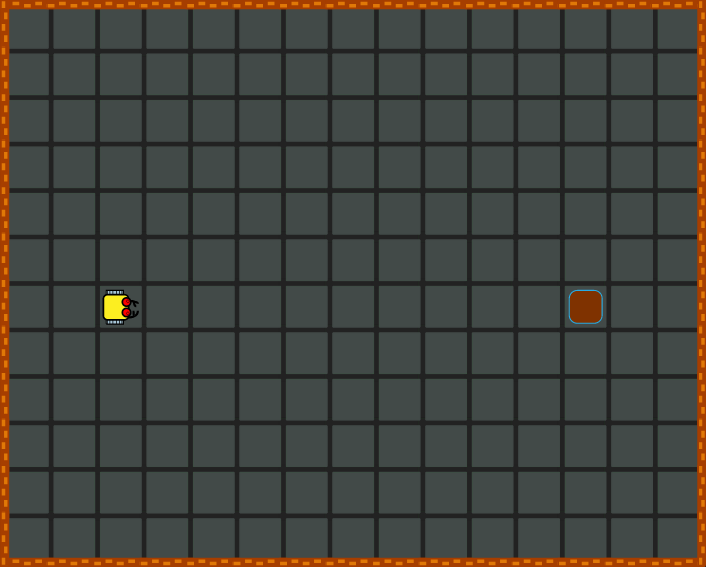
\includegraphics[width=0.7\textwidth]{img/c01.png}
\end{center}
\vspace{-4mm}
\caption{Karel gets home elegantly, using the {\tt repeat} command.}
\label{fig:c01}
\vspace{-4mm}
\end{figure}
\noindent

\newpage

\subsection{Exercise C02 - Lucky Strike}

{\em Karel is about to find a pile of 12 gems! Write a program for the robot to collect the gems and get home. Use the {\tt repeat} command for any repeated action. 

\begin{figure}[!ht]
\begin{center}
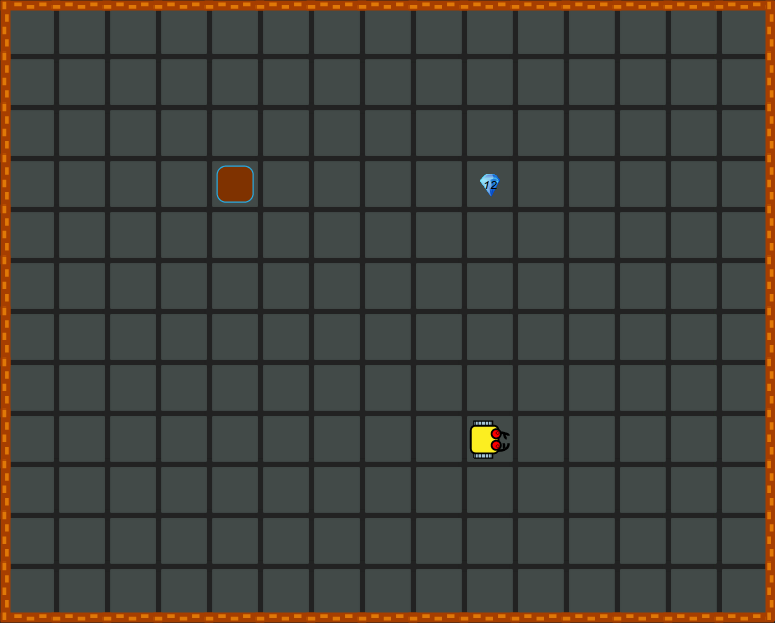
\includegraphics[width=0.7\textwidth]{img/c02.png}
\end{center}
\vspace{-4mm}
\caption{Karel is about to find a pile of 12 gems!}
\label{fig:c02}
\vspace{-4mm}
\end{figure}
\noindent


\subsection{Exercise C03 - Feelin' Lucky}

{\em Karel is feeling lucky today. He wants to just step outside his house, 
turn around five times, then pick up one gem somewhere, and get back inside!}


\begin{figure}[!ht]
\begin{center}
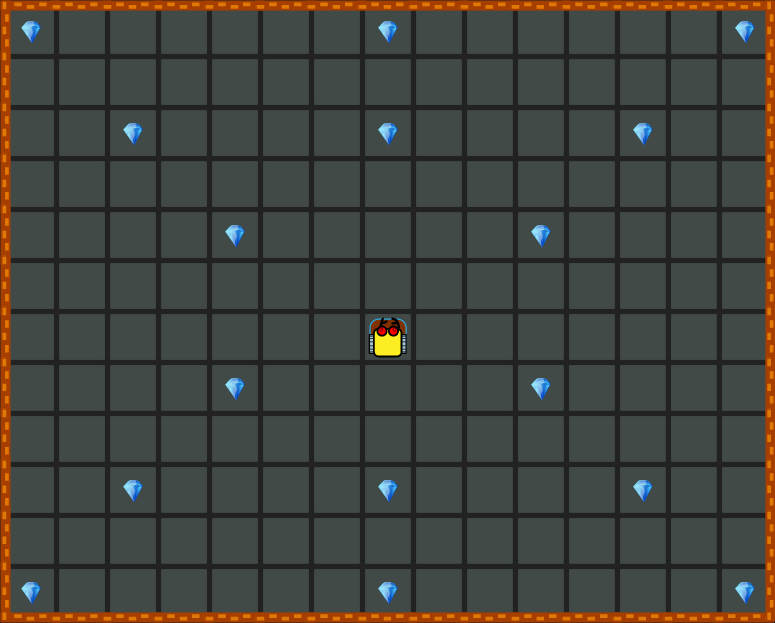
\includegraphics[width=0.7\textwidth]{img/c03.png}
\end{center}
\vspace{-4mm}
\caption{Karel is feeling lucky today.}
\label{fig:c03}
\vspace{-4mm}
\end{figure}
\noindent


\subsection{Exercise C04 - Garage Sale}

{\em Karel needs to sell 10 of his oldest gems in order to make space for new ones. 
Write a program for the robot to step out of his garage, put 10 gems on the ground, 
and then turn back and get back inside! Use the {\tt repeat} command for any repeated 
action.}


\begin{figure}[!ht]
\begin{center}
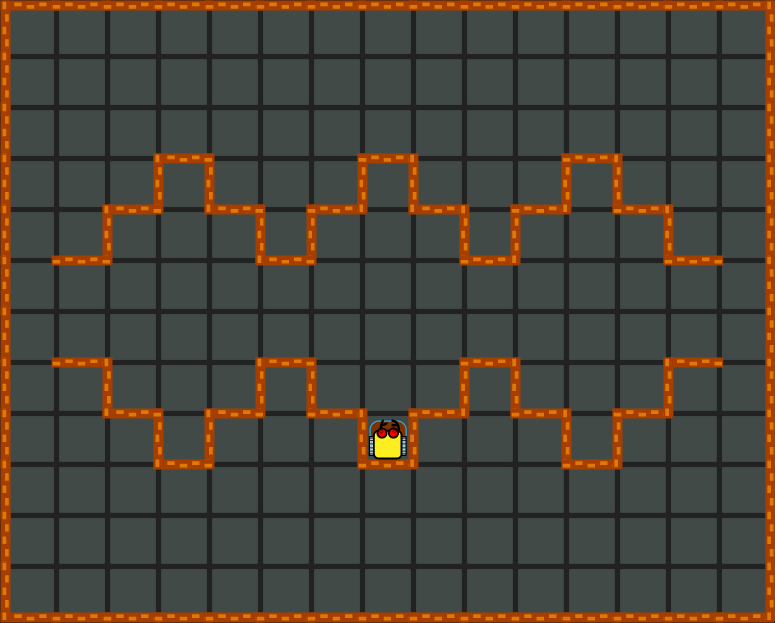
\includegraphics[width=0.7\textwidth]{img/c04.png}
\end{center}
\vspace{-4mm}
\caption{Karel is getting ready for garage sale.}
\label{fig:c04}
\vspace{-4mm}
\end{figure}
\noindent



\subsection{Exercise C05 - String of Gems}

{\em Write a program for Karel to collect all nine gems and get home! 
Writing one command per line, your program should not have more 
than three lines.}.

\newpage
\begin{figure}[!ht]
\begin{center}
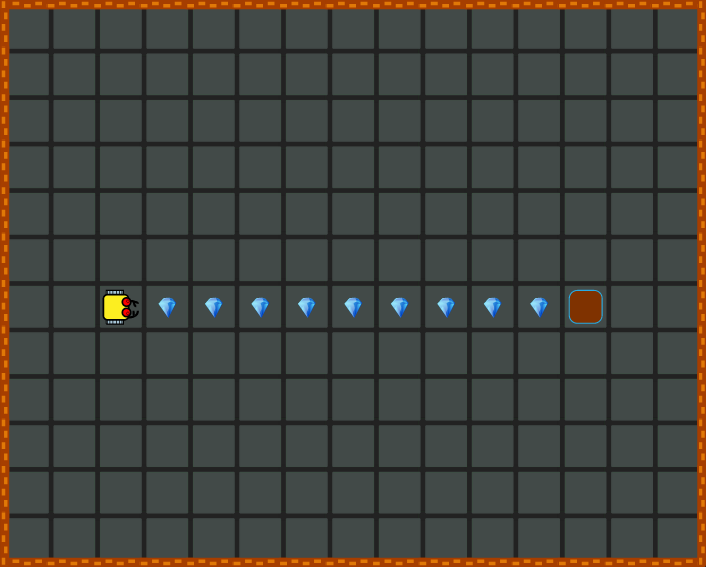
\includegraphics[width=0.7\textwidth]{img/c05.png}
\end{center}
\vspace{-4mm}
\caption{Nine gems are between Karel and his home.}
\label{fig:c05}
\vspace{-10mm}
\end{figure}
\noindent

\section{Intermission - Working with Input and Text Cells} \label{sec:editmenu}

\subsection{Objectives} 
 
\begin{itemize}
\item Learn why descriptive text cells are useful and how to insert them.
\item Learn when it makes sense to have multiple input cells and how to add them.
\item Learn how to run all input cells at once, and how to run them individually.
\item Learn how to clear, remove and merge cells.
\end{itemize}
There are a couple of simple new rules to remember:
\begin{enumerate} 
\item Programs are entered into input cells on the left (one will appear after you press Start).
\item Always type one command per line -- this does not hold only for Karel but for any
      programming language. It makes computer code much easier to read.
\item Clicking on "clear" under an input cell will erase its contents.
\item You can add a new input cell by clicking on "add" (located under each input cell). 
      Having multiple input cells can be useful, for example, to test various versions 
      of your program, or if you want to run parts of your program separately. 
\item Clicking on "remove" under an input cell will remove it. All text in that cell will be lost.
\item Run programs via the blue arrow button in the menu (this will evaluate all input
      cells). Each cell can be evaluated individually by clicking on "run" (located under 
      each input cell). If there is just one input cell, both options are equivalent.
\item Running programs can be stopped using the blue square button in the menu.
\end{enumerate}

\subsection{Review questions}

\begin{enumerate}
\item Where do we enter programs for Karel?
\begin{enumerate}
\item[A1] In Microsoft Word.
\item[A2] In DreamWeaver.
\item[A3] We upload them from hard disk.
\item[A4] In input cells.
\end{enumerate}
\item How many commands per line should we type?
\begin{enumerate}
\item[A1] At least two.
\item[A2] As many as possible.
\item[A3] Only one.
\item[A4] At most five.
\end{enumerate}
\item How can we add a new input cell?
\begin{enumerate}
\item[A1] Clicking on "add" under an existing input cell.
\item[A2] Through "Add new input cell" in the Edit menu.
\item[A3] Through "New" in File menu.
\item[A4] Through "Clone" in File menu.
\end{enumerate}
\item When should we have multiple input cells?
\begin{enumerate}
\item[A1] When our program contains more than one command.
\item[A2] When we want to run parts of the program separately.
\item[A3] When a command is repeated multiple times.
\item[A4] When the program is longer than 10 lines.
\end{enumerate}
\item What do we need to do in order to erase all text from an input cell?
\begin{enumerate}
\item[A1] Close Karel, logout from NCLab and login again. 
\item[A2] Restart Karel.
\item[A3] Remove the input cell and add a new one in its place.
\item[A4] Click on "clear" under the input cell.
\end{enumerate}
\item How can we remove an input cell?
\begin{enumerate}
\item[A1] Click on "add" under the input cell.
\item[A2] Click on "remove" under the input cell.
\item[A3] Click on "clear" under the input cell.
\item[A4] Switch to Build mode and back.
\end{enumerate}
\item How can we evaluate all input cells at once?
\begin{enumerate}
\item[A1] Through "Expand all cells" in Edit menu.
\item[A2] Click on the blue square button.
\item[A3] Click on "run" under the last input cell.
\item[A4] Click on the blue arrow button.
\end{enumerate}
\item How should running programs be stopped?
\begin{enumerate}
\item[A1] Click on the blue arrow button.
\item[A2] Close the main Karel window.
\item[A3] Click on the blue square button.
\item[A4] Click on "stop" under the last input cell.
\end{enumerate}
\item How can we evaluate just one selected input cell?
\begin{enumerate}
\item[A1] We have to copy and paste the contents of all 
          input cells into the first one, and remove them.
\item[A2] Clicking on the blue arrow button in the menu. 
\item[A3] Clicking on "run" under the input cell.
\item[A4] Clicking on "remove" under the input cell.
\end{enumerate}
\end{enumerate}




\section{Section D - Conditions}

\subsection{Objectives} 

\begin{itemize}
\item Understand the function of Karel's five sensors.
\item Learn to use the sensors in conjunction with {\em conditions} to help Karel 
      check his surroundings and react accordingly. For example, you will learn to first 
      check whether wall is ahead before making a step forward, checking whether there
      is a gem on the ground before attempting to pick it up, etc.
\end{itemize}

\noindent
Karel has built-in sensors to better navigate in the maze:

\subsection{Karel's five sensors}

The first one is an infrared sensor that the robot uses to determine 
whether it is safe to make one step forward, or whether there is a wall.
The usage can be illustrated using a simple program "Careful step" 
where Karel first checks whether there is a wall ahead before
making a step. If there is wall, he turns back: 

\begin{verbatim}
# Program "Careful step".
if wall
  repeat 2
    left
else
  go
\end{verbatim}
Note that the symbol {\tt \#} introduces a comment, meaning that the line 
of code behind it is ignored by the robot.
The {\tt else} branch does not have to be there if it is not needed. Notice the indentation 
of the bodies of the {\tt if} and {\tt else} branches - this is analogous 
to how we indent the body of the {\tt repeat} command.

Besides {\tt wall}, the robot can check the following:
\begin{itemize}
\item {\tt gem} ... is there a gem where he stands?
\item {\tt empty} ... is his bag with gems empty?
\item {\tt north} ... is he facing North?
\item {\tt home} ... is he at home?
\end{itemize}
Karel can also use the reserved word {\tt not} to test the opposites.
For illustration, the previous program can be rewritten as follows, without changing its function:
\begin{verbatim}
# Program "Careful step".
if not wall
  go
else
  repeat 2
    left
\end{verbatim}

\subsection{Programming wisdom}

Good programmer is a careful programmer! Errors can be avoided by always checking the 
appropriate sensor before making an action. A few examples of careful actions:
 
\begin{verbatim}
if not wall
  go
\end{verbatim}
Another example:
 
\begin{verbatim}
if gem
  get
\end{verbatim}
And a last one:
 
\begin{verbatim}
if not empty
  put
\end{verbatim}


\subsection{Review questions}

\begin{enumerate}
\item What are the five sensors that Karel can use, and what do they do?
\item Can he  see from where he stands whether a wall is two steps ahead?
\item Can he check without turning whether a wall is on his right?
\item Can he check from where he stands whether a gem is one step away?
\item Can he check from where he stands whether his home is one step away?
\item Can he check whether he has at least one gem in the bag?
\item Can he check without turning whether he faces West?
\item Write a program for Karel to check whether Karel stands on a gem, and if so, to pick it up.
\item Write a program for Karel to check whether his bag is not empty, and if not, to put one gem on the ground. 
\item Write a program for Karel to turn North. 

\end{enumerate}

\subsection{Exercise D01 - In the Fog}

{\em Several gems lie on the ground between the robot and his home which is 10 steps away. 
He cannot see where they are exactly since his sensor only tells him if a gem is right 
under him.  And besides that, nothing is visible in today's foggy weather anyway. 
Write a program for Karel to collect all gems and get home. With one command per 
line, your program should have at most 4 lines.}


\begin{figure}[!ht]
\begin{center}
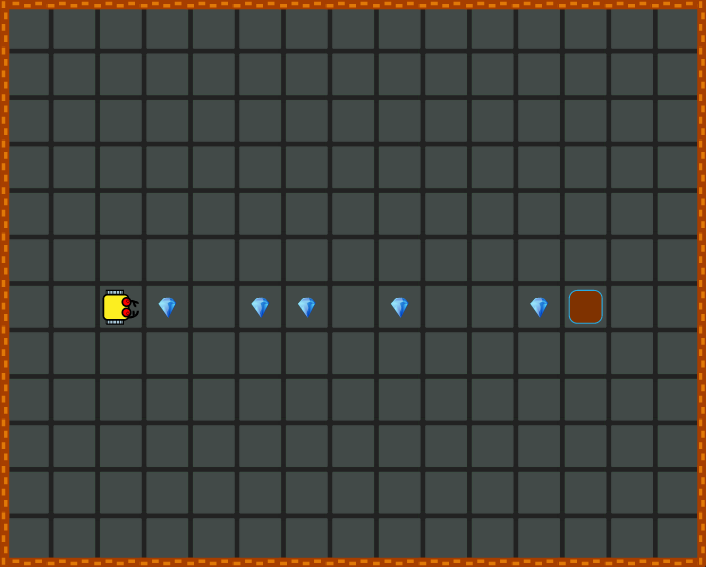
\includegraphics[width=0.7\textwidth]{img/d01.png}
\end{center}
\vspace{-4mm}
\caption{With zero visibility, Karel needs to rely on his sensors.}
\label{fig:d01}
\vspace{-4mm}
\end{figure}
\noindent

\newpage

\subsection{Exercise D02 - Stony Meadows}

{\em Karel is walking on a meadows that is covered with irregularly 
scattered stones. Write a program for the robot to get to his home, 
avoiding stones, and collecting all three gems!  }


\begin{figure}[!ht]
\begin{center}
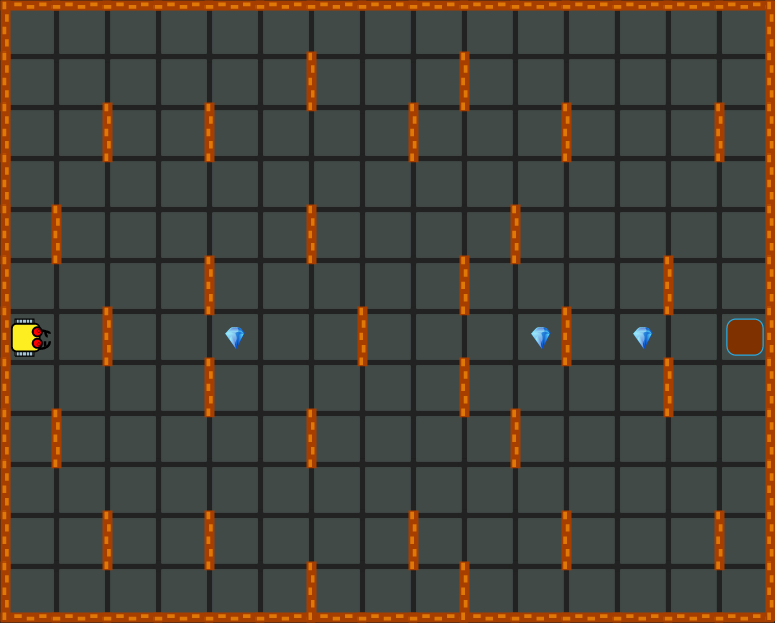
\includegraphics[width=0.7\textwidth]{img/d02.png}
\end{center}
\vspace{-4mm}
\caption{Karel is crossing a stony meadows.}
\label{fig:d02}
\vspace{-4mm}
\end{figure}
\noindent





\subsection{Exercise D03 - Filling the Blanks}

{\em Karel stores all his gems in a secret chest in his cellar. 
Currently, some shelves are empty. Write a program for Karel to 
inspect all shelves and put a gem where one is missing! After that, he needs to get 
home as usual. With one 
command per line, your program should have at most 7 lines.}

\begin{figure}[!ht]
\begin{center}
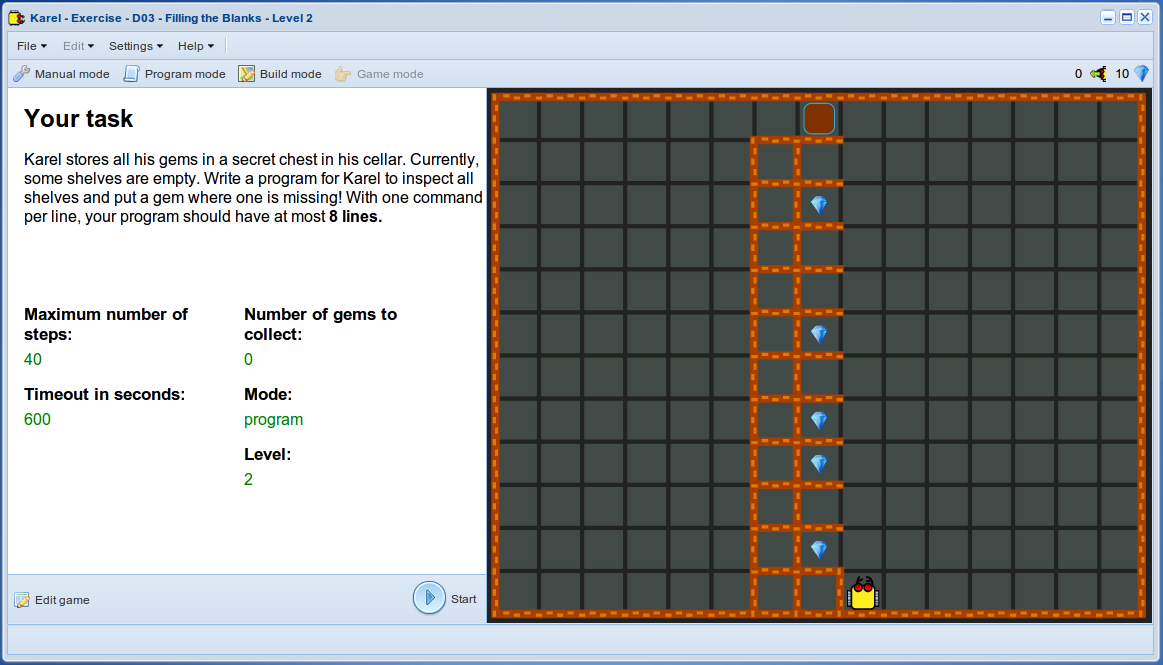
\includegraphics[width=0.7\textwidth]{img/d03.png}
\end{center}
\vspace{-4mm}
\caption{Filling empty shelves with gems.}
\label{fig:d03}
\vspace{-4mm}
\end{figure}
\noindent



\section{Section E - Conditional Loop}

\subsection{Objectives} 
 
\begin{itemize}
\item Learn to repeat a command or a sequence of commands when it is not known 
      how many repetitions will be needed.
\end{itemize}

\noindent
In this section we will learn another type of loop that is highly useful 
in programming.

\subsection{The {\tt while} command}

Often Karel needs to repeat something, {\em not knowing in advance how many repetitions
there will be}. This can be the case, for example, 
when he is asked to walk straight ahead until he reaches the closest wall.
Remember that he only can see walls that are right ahead of him; walls 
that are further away he can't see. Such a program would be:

\begin{verbatim}
while not wall
  go
\end{verbatim}
Or, he may be asked to walk until he gets home:

\begin{verbatim}
while not home
  go
\end{verbatim}
Or, he may be asked to empty his bag (he does not know how many gems are in it): 
 
\begin{verbatim}
while not empty
  put
\end{verbatim}
Or, he may be asked to collect all gems from a pile (he does not know 
how many gems there are):

\begin{verbatim}
while gem
  get
\end{verbatim}
Or we may ask him to turn to face North (he does not know which direction he is
facing):

\begin{verbatim}
while not north
  left
\end{verbatim}
At last, Karel is asked to 
turn South, walk straight ahead until he reaches the closest wall, and 
collect all gems that he can find on the way:

\begin{verbatim}
# First turn North.
while not north
  left

# Then turn South.
repeat 2
  left

# Go straight ahead and pick all gems.
while not wall
  if gem
    get
  go

# Pick gem at the wall (if any).
if gem
  get
\end{verbatim}
Notice that we first need to turn the robot to face North -- this is because North 
is the only direction that he can check!

\subsection{Review questions}

\begin{enumerate}
\item What is the difference between the {\tt repeat} and {\tt while} loops?
\item Write a program for Karel to turn North {\em not using} the {\tt while} loop. 
\item Then write a program for Karel to turn North {\em using} the {\tt while} loop. 
      Compare the length and elegance of this program with the one from the 
      previous question.
\end{enumerate}

\subsection{Exercise E01 - South West}

{\em Karel is lost and he does not even know whether he is facing north, south, east or west! He only knows that his home is in the south-west corner of the maze. Write a program for the robot to get there. Hint: First you need to orient the robot to face north, that's the only direction that he can check with his sensors.}


\begin{figure}[!ht]
\begin{center}
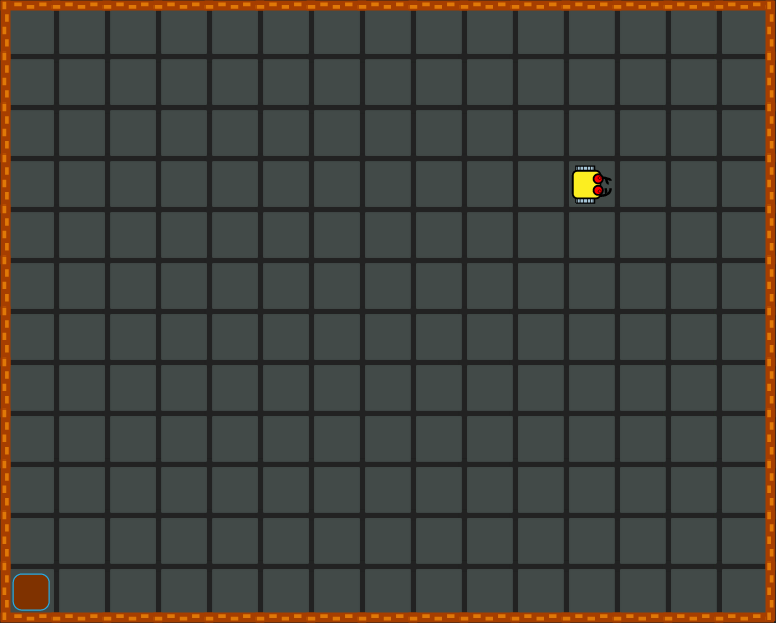
\includegraphics[width=0.7\textwidth]{img/e01.png}
\end{center}
\vspace{-4mm}
\caption{Karel only knows that his home is in the SW corner of the maze.}
\label{fig:e01}
%\vspace{-12mm}
\end{figure}
\noindent


\subsection{Exercise E02 - Hide-and-Seek}

{\em Karel's friends are hiding. He knows that he has to go straight 
ahead to find them. When he finds a gem, he has to turn left and keep 
walking. Eventually, he will get to the place where his friends are 
hiding. If he gets home, stop. Write a program for Karel to do this, 
and do not forget to collect all the gems on the way!}

\newpage

\begin{figure}[!ht]
\begin{center}
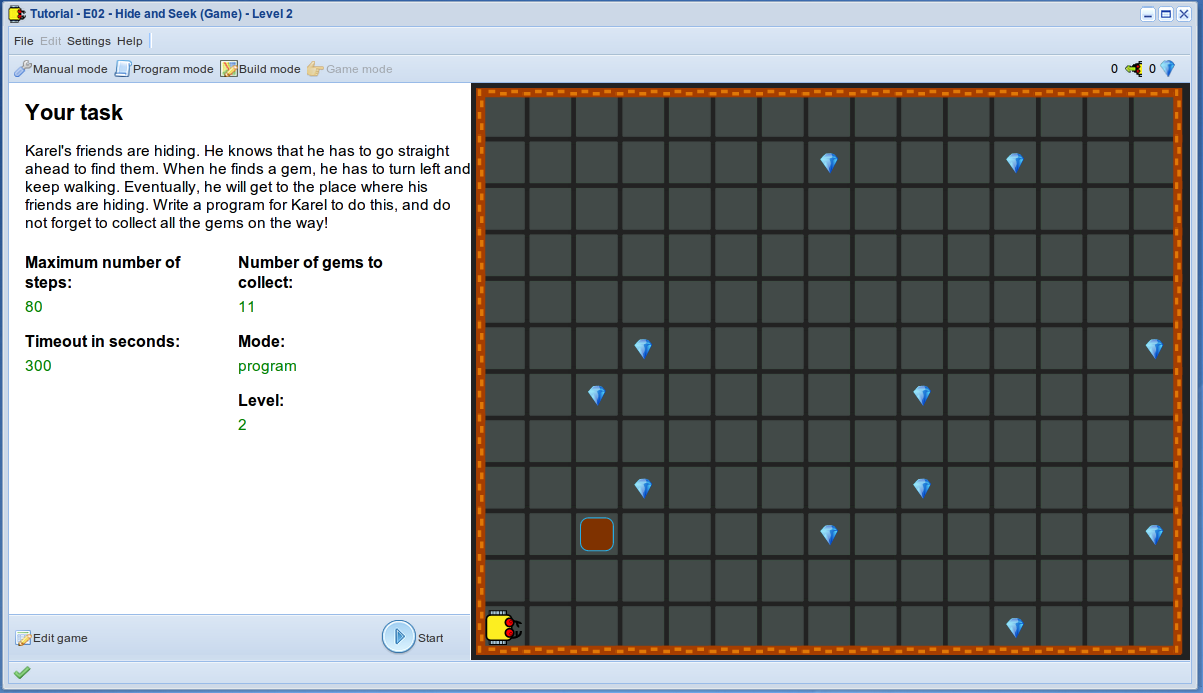
\includegraphics[width=0.7\textwidth]{img/e02.png}
\end{center}
\vspace{-4mm}
\caption{Karel plays hide-and-seek with his friends.}
\label{fig:e02}
\end{figure}
\noindent

\subsection{Exercise E03 - Walk the Line}

{\em Karel stands next to a straight wall and he knows that his home is somewhere on the other side of it. He does not know how long the wall is, nor the exact position of his home. Write a program for the robot to get there!}

\begin{figure}[!ht]
\begin{center}
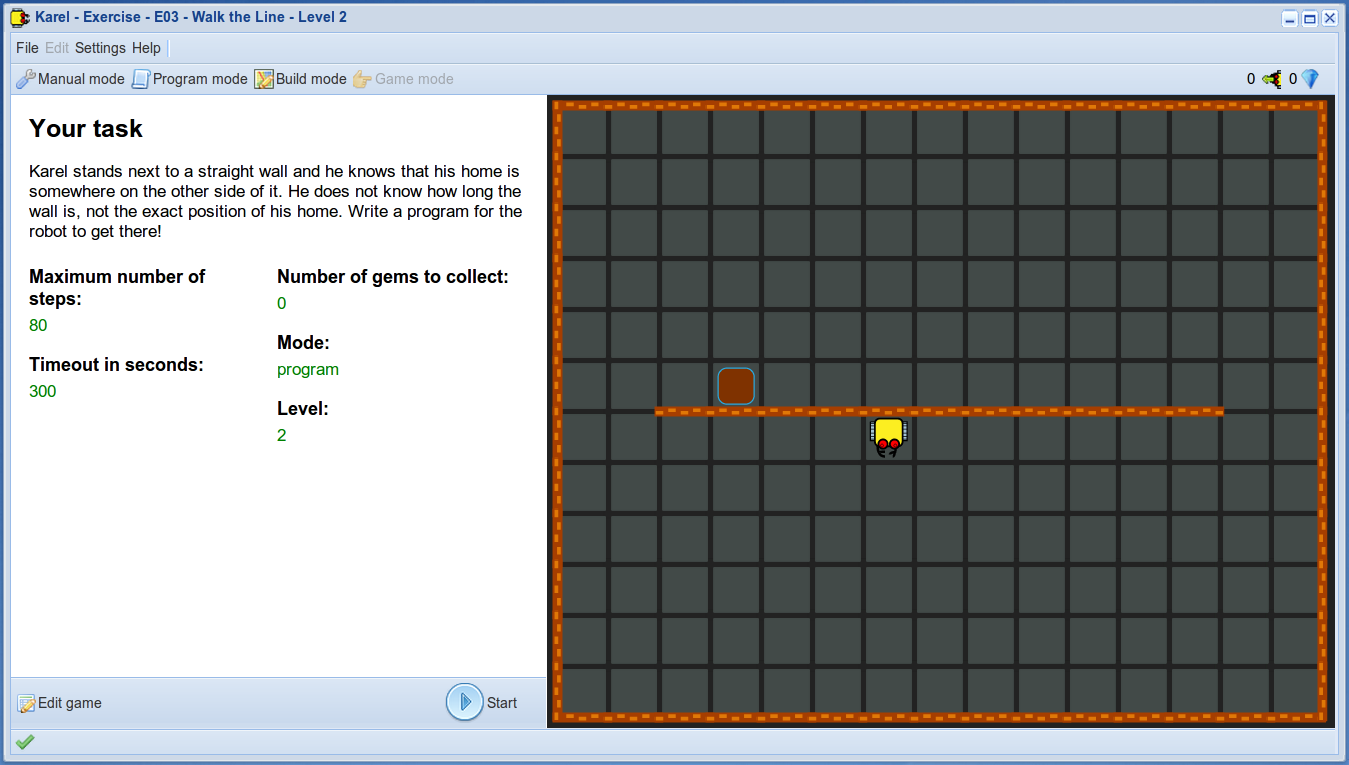
\includegraphics[width=0.7\textwidth]{img/e03.png}
\end{center}
\vspace{-4mm}
\caption{Karel only knows that his home is on the other side of the wall.}
\label{fig:e03}
\vspace{-10mm}
\end{figure}
\noindent

\newpage

\section{Section F - Defining New Commands}

\subsection{Objectives} 
 
\begin{itemize}
\item Learn to never copy and paste computer code.
\item Learn to recognize smaller tasks that can be solved without solving the big task.
\item Learn to bring more structure and clarity into your programs by introducing new commands.
\end{itemize}

\subsection{Programming wisdom}

{\em Always look for small tasks that can be solved independently of the big ones.
Solve the small tasks first, and you'll see that the big ones get much simpler. The 
importance of what we just said cannot be stressed more. Please read these three 
lines once more.}\\

\noindent
The fact that you are reading this line of text proves that you are not 
a perfect programmer yet. Otherwise you would be stuck forever in the 
previous infinite loop!

\begin{figure}[!ht]
\begin{center}

\includegraphics[width=0.3\textwidth]{img/smiley.png}
\end{center}
\vspace{-1cm}
\end{figure}


\subsection{More programming wisdom}

A new command should be defined whenever it becomes clear that the same 
action is repeated in the algorithm multiple times (yes, we talk about the algorithm,
not about the program). If you start writing a program and then realize that the same
code repeats itself at various places, then probably you did not do a good job 
designing the algorithm.

Sometimes it might be 
tempting to just copy and paste the same code several times in the 
program, because it does the same thing, but never do it! This would be very bad programming
and sooner or later your own code would punish you for that. 
You would make a small change at one place but forget to do it 
in all the other places. Then your code would start 
acting strange, it would sometimes work and sometimes fail. 
You would spend lots of time looking for the mistakes, find some 
of them but not all, and your program would become unreliable
and after some time irreparable. You would find that you need to 
rewrite it from scratch.

\subsection{Defining new commands}

New commands are defined using the reserved word 
{\tt def}. For example, in a program where the robot needs to turn back
many times, it is a good idea to define a new command {\tt back}
as follows:

\begin{verbatim}
def back
  repeat 2
    left
\end{verbatim}
Note the indent -- the body of a new command needs to be indented 
analogously to the bodies of loops and conditions.

\subsection{Revisiting exercise A07}

Let us return to the exercise A07 - Right Button for a moment.
A really bad program to solve this task would be:

{\small
\begin{verbatim}
right
go
go
go
go 
get
right
go
go
go
go 
get
right
go
go
go
go
get
\end{verbatim}
}
\noindent
Can you see how many times the same code is repeated?! In order to fix this, 
we should define new command {\tt foursteps} as
follows:

{\small
\begin{verbatim}
def foursteps
  repeat 4
    go
\end{verbatim}
}
\noindent
With this new command, the above code simplifies to 

{\small
\begin{verbatim}
right
foursteps
get
right
foursteps
get
right
foursteps
get
\end{verbatim}
}
\noindent
There are still repetitions that must be eliminated! So we define a new command 
{\tt walkedge}:

{\small
\begin{verbatim}
def walkedge
  right
  foursteps
  get
\end{verbatim}
}
\noindent
Now with the new commands {\tt foursteps} and
{\tt walkedge}, our program simplifies to:

{\small
\begin{verbatim}
while not home
  walkedge
\end{verbatim}
}
\noindent
It is the task of the first exercise in this Section to implement this program. But before we 
do so, let us mention one very important thing.

\subsection{Solution procedure revisited (and corrected)}

Let's forget the commands that we defined above.
Experienced programmer would never approach the problem the way we did.
He (or she but let's use "he" for simplicity) 
would first look at the problem, trying to recognize repeating patterns. 
He would find that the task can be fulfilled by repeating one simpler task 
three times. So, without knowing exactly how the smaller task is going to 
be solved, he would write:

{\small
\begin{verbatim}
while not home
  walkedge
\end{verbatim}
}
\noindent
Next he would define the new command {\tt walkedge} as follows:

{\small
\begin{verbatim}
def walkedge
  right
  foursteps
  get
\end{verbatim}
}
\noindent
He would not bother defining the command 
{\tt foursteps} yet, because he knows that this will be 
simple. And as the last step, to make the program work, he would 
define:

{\small
\begin{verbatim}
def foursteps
  repeat 4
    go
\end{verbatim}
}

\subsection{Review questions}

\begin{enumerate}
\item When should a new command be defined?
\item What will happen when we copy and paste the same code 
      to multiple places in our program?
\item Write a new command {\tt emptybag} that empties Karel's bag.
\item Write a new command {\tt turnsouth} that turns Karel to the South no matter 
      which direction he is facing.
\end{enumerate}


\subsection{Exercise F01 - Four Star Hotel}

{\em Before getting home, Karel has to collect all four stars of gems!}


\begin{figure}[!ht]
\begin{center}
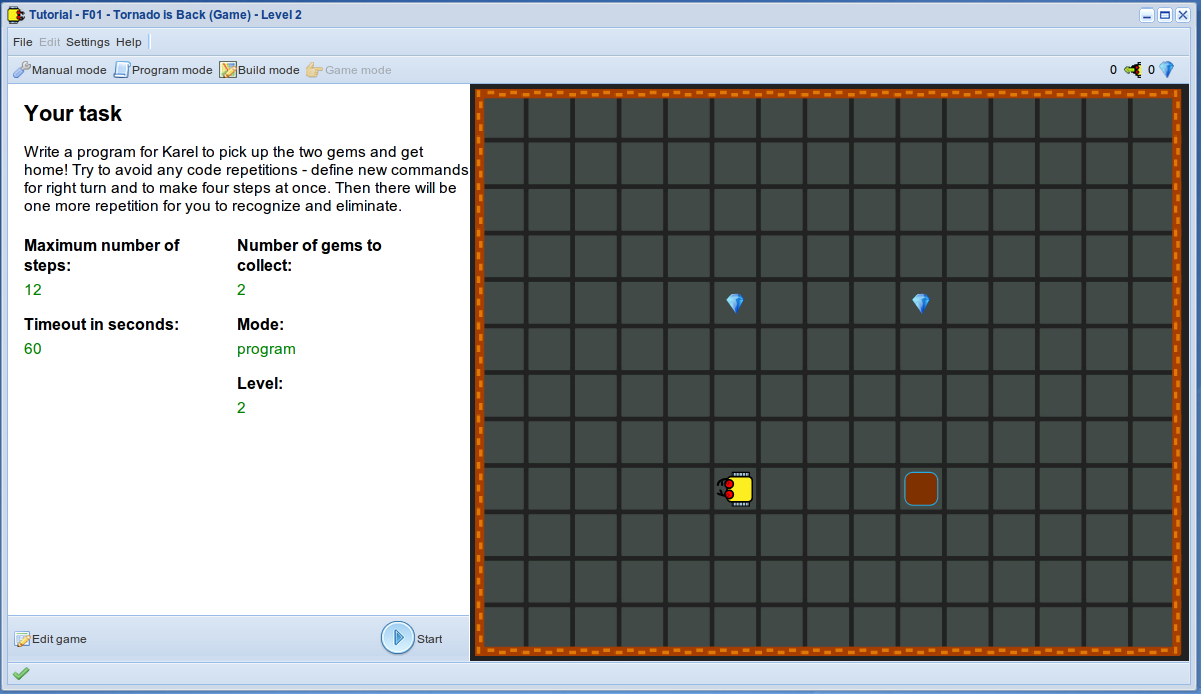
\includegraphics[width=0.7\textwidth]{img/f01.png}
\end{center}
\vspace{-4mm}
\caption{Karel needs to collect four stars of gems.}
\label{fig:f01}
\vspace{-10mm}
\end{figure}
\noindent

\subsection{Exercise F02 - U-Haul}

{\em Write a program for the robot to move the 6x6 square of gems to the opposite corner of the maze. The task is finished when the robot is back home.}
\newpage

\begin{figure}[!ht]
\begin{center}
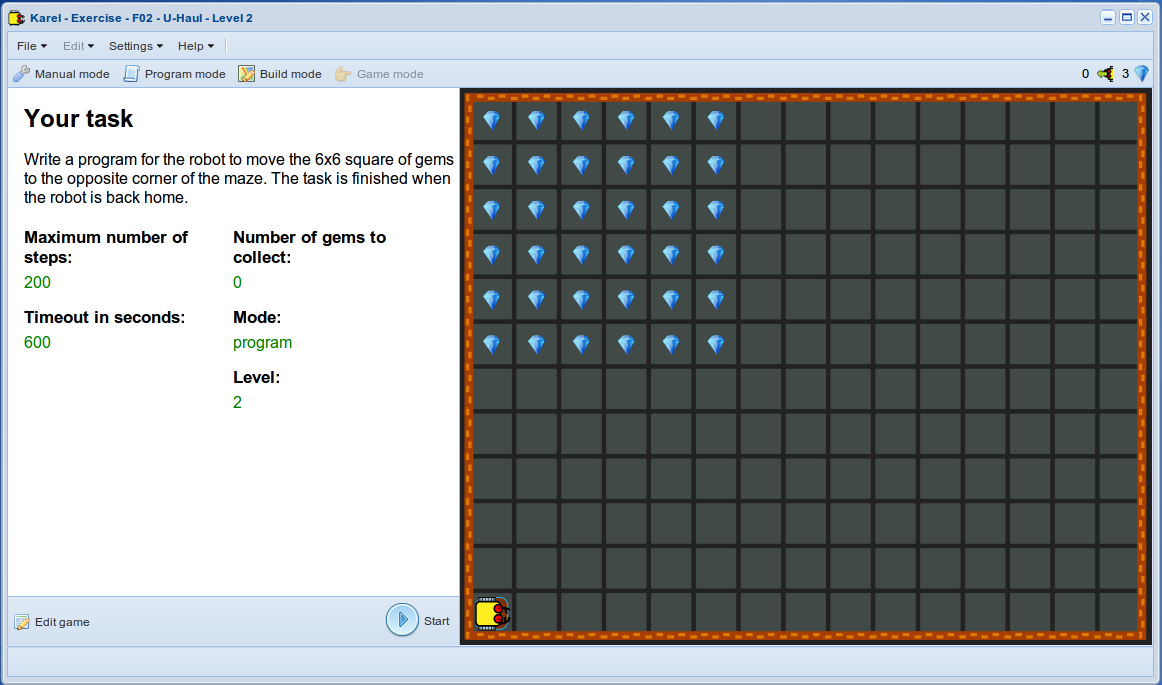
\includegraphics[width=0.7\textwidth]{img/f02.png}
\end{center}
\vspace{-4mm}
\caption{Karel needs to move the gems to the opposite corner of the maze.}
\label{fig:f02}
\vspace{-10mm}
\end{figure}
\noindent

\subsection{\ \ Exercise F03 - Egg Hunt}

{\em Write a program for Karel to search all cells and collect all eggs (gems) that he can find. The task is finished when the robot is back home.}


\begin{figure}[!ht]
\begin{center}
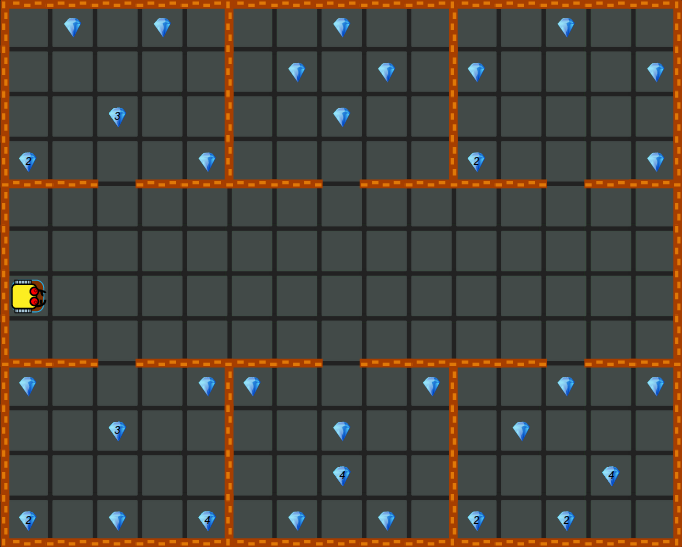
\includegraphics[width=0.7\textwidth]{img/f03.png}
\end{center}
\vspace{-4mm}
\caption{Easter is here, Karel is on egg hunt!}
\label{fig:f03}
\vspace{-10mm}
\end{figure}
\noindent

\subsection{\ \ Exercise F04 - Blind Carpenter}

{\em Karel is a blind carpenter who needs to install windows (gems) into a newly built house. All he knows is that the house is a rectangle and that each window is exactly one tile large, But he can't see where the openings for the windows are. Install the windows and return home!}


\begin{figure}[!ht]
\begin{center}
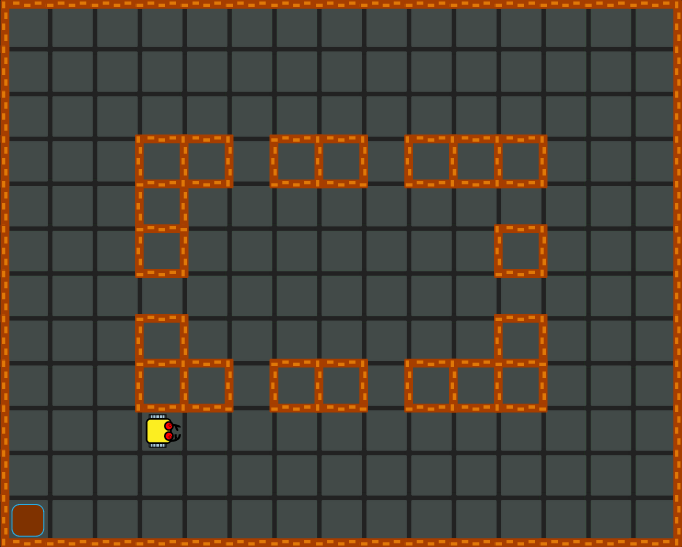
\includegraphics[width=0.7\textwidth]{img/f04.png}
\end{center}
\vspace{-4mm}
\caption{This time Karel installs windows.}
\label{fig:f04}
%\vspace{-10mm}
\end{figure}
\noindent



\subsection{\ \ Exercise F05 - Pirate Ship}

{\em Karel is on a pirate ship! Write a program for him to collect all 
gems and run away (to his home) before the pirates are back. Here Karel 
needs to be extremely efficient to survive. Therefore, there should be 
no repeating parts whatsoever in your program!}


\begin{figure}[!ht]
\begin{center}
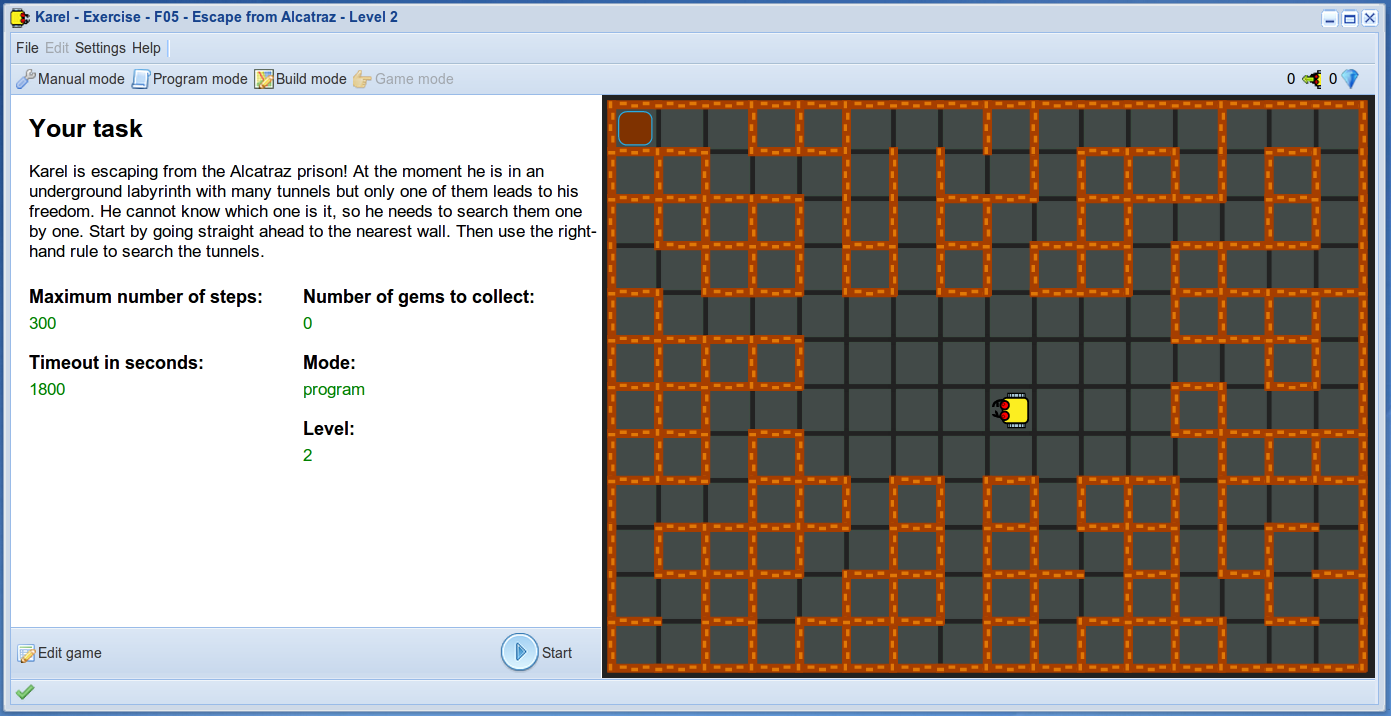
\includegraphics[width=0.7\textwidth]{img/f05.png}
\end{center}
\vspace{-4mm}
\caption{Karel found a pirate treasure.}
\label{fig:f05}
\vspace{-10mm}
\end{figure}
\noindent

\newpage
\subsection{\ \ Exercise F06 - Diamond Staircase}

{\em Write a program for Karel to climb the stairs, collect all gems, and get home!}


\begin{figure}[!ht]
\begin{center}
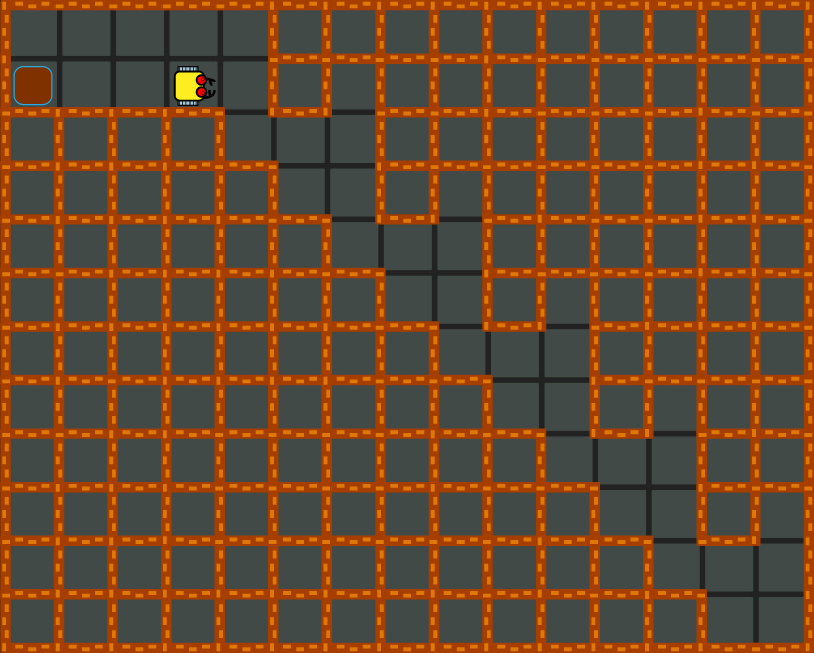
\includegraphics[width=0.7\textwidth]{img/g01.png}
\end{center}
\vspace{-4mm}
\caption{This time Karel has to do some climbing.}
\label{fig:g01}
\vspace{-4mm}
\end{figure}
\noindent


\subsection{\ \ Exercise F07 - Plucking Flowers}

{\em Write a program for Karel to pluck all flowers that grow at the fence of his garden (gems), and get back home! Note two level of repetitions - the fence has four edges, and it takes 7 steps to walk each edge.}


\begin{figure}[!ht]
\begin{center}
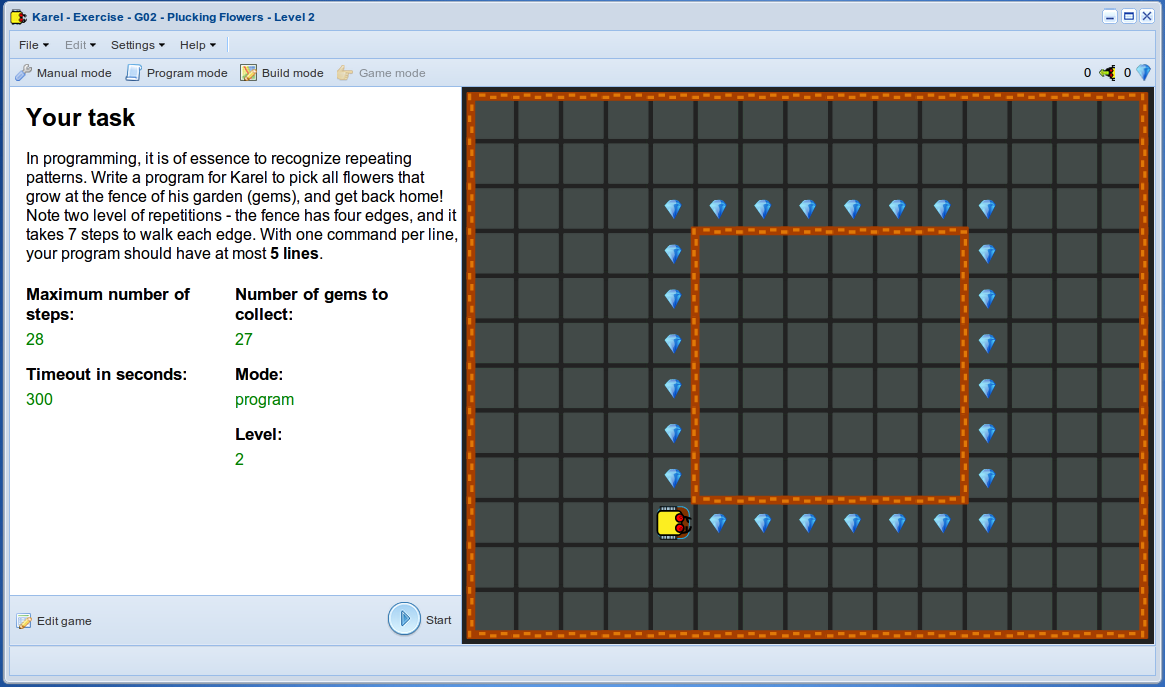
\includegraphics[width=0.7\textwidth]{img/g02.png}
\end{center}
\vspace{-4mm}
\caption{Karel is plucking flowers along his fence.}
\label{fig:g02}
\vspace{-4mm}
\end{figure}
\noindent

\subsection{\ \ Exercise F08 - Gems for Friends}

{\em Karel has three gems in his bag, that he wants to give to his three friends R2, D2 and Marvin who live close by. They are very good friends, so Karel is allowed to enter their homes at any time. Write a program for Karel to put a gem on the ground in the middle of each friend's home, and then get back to his own house! Hint: There will be an outer loop of four repetitions, that will contains inner repetitions in it.}


\begin{figure}[!ht]
\begin{center}
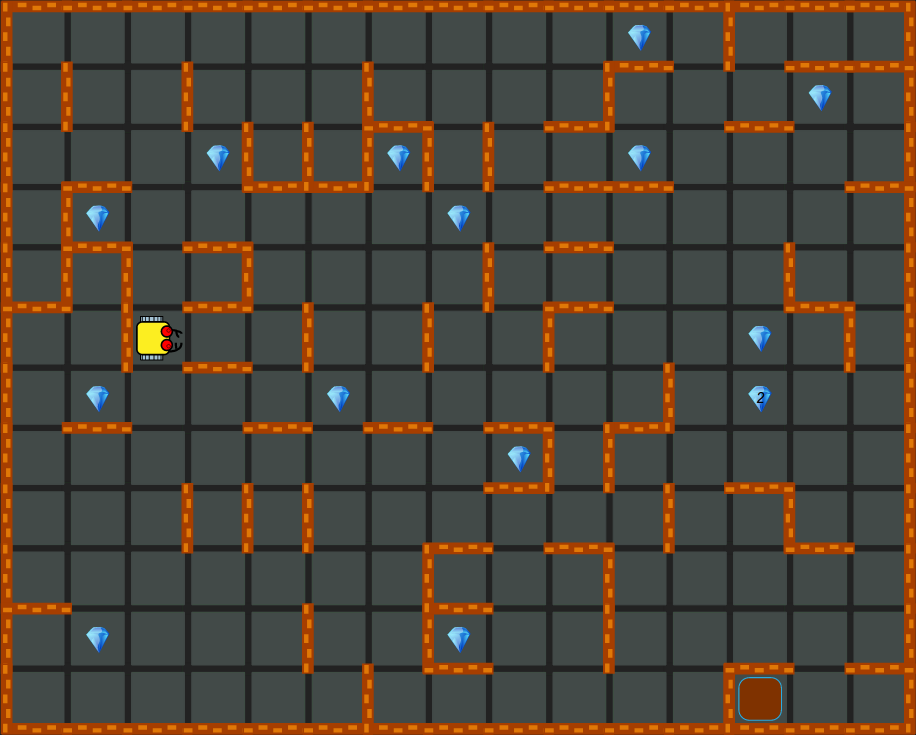
\includegraphics[width=0.7\textwidth]{img/g03.png}
\end{center}
\vspace{-4mm}
\caption{Karel is going to give gems to his three friends R2, D2 and Marvin.}
\label{fig:g03}
\vspace{-4mm}
\end{figure}
\noindent

\subsection{\ \ Exercise F09 - Diamond Rectangle}

{\em Karel stands in front of a rectangle with unknown dimensions. He knows that the rectangle is surrounded with gems. Sometimes the gems are piled up, but he does not know how many gems are in each pile. Write a program for the robot to walk around the rectangle, collect all gems, and get home!}

\newpage

\begin{figure}[!ht]
\begin{center}
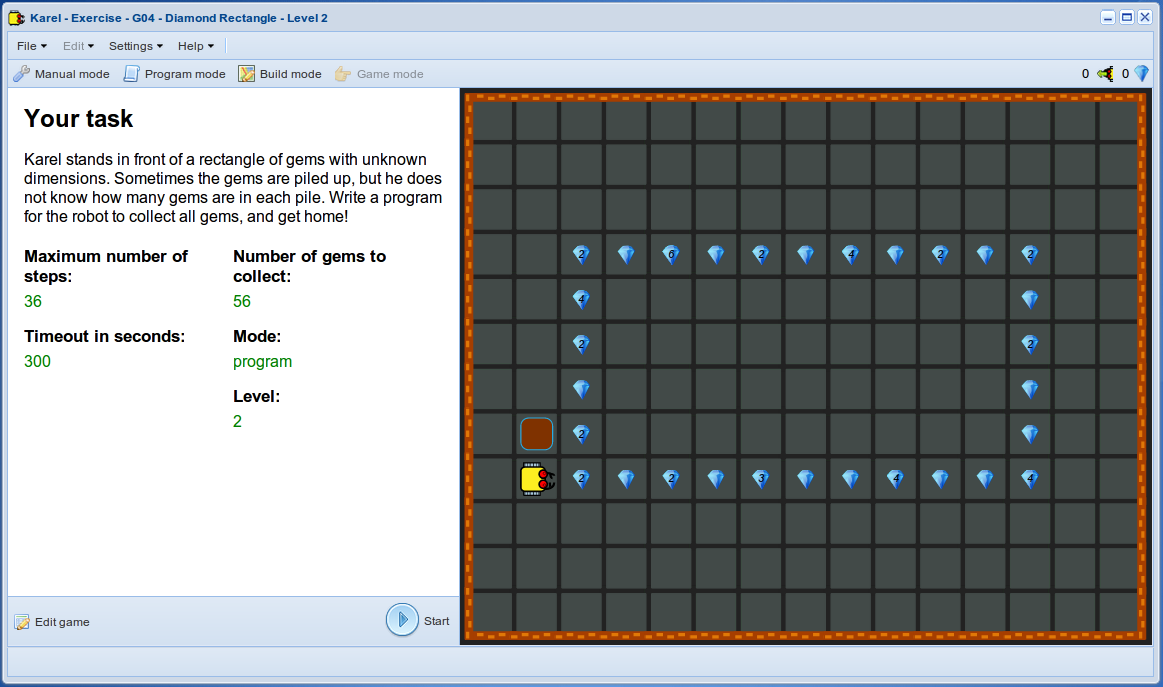
\includegraphics[width=0.7\textwidth]{img/g04.png}
\end{center}
\vspace{-4mm}
\caption{This time Karel does not know the size of the rectangle.}
\label{fig:g04}
\vspace{-10mm}
\end{figure}
\noindent

\subsection{\ \ Exercise F10 - Gem Jam!}

{\em In this maze, gems are distributed randomly along the walls. Otherwise 
the maze is empty. Karel's home is in the south-west corner, and the robot 
stands on the right of it, facing east. Write a program for Karel to collect 
all the gems and return home!}

\begin{figure}[!ht]
\begin{center}
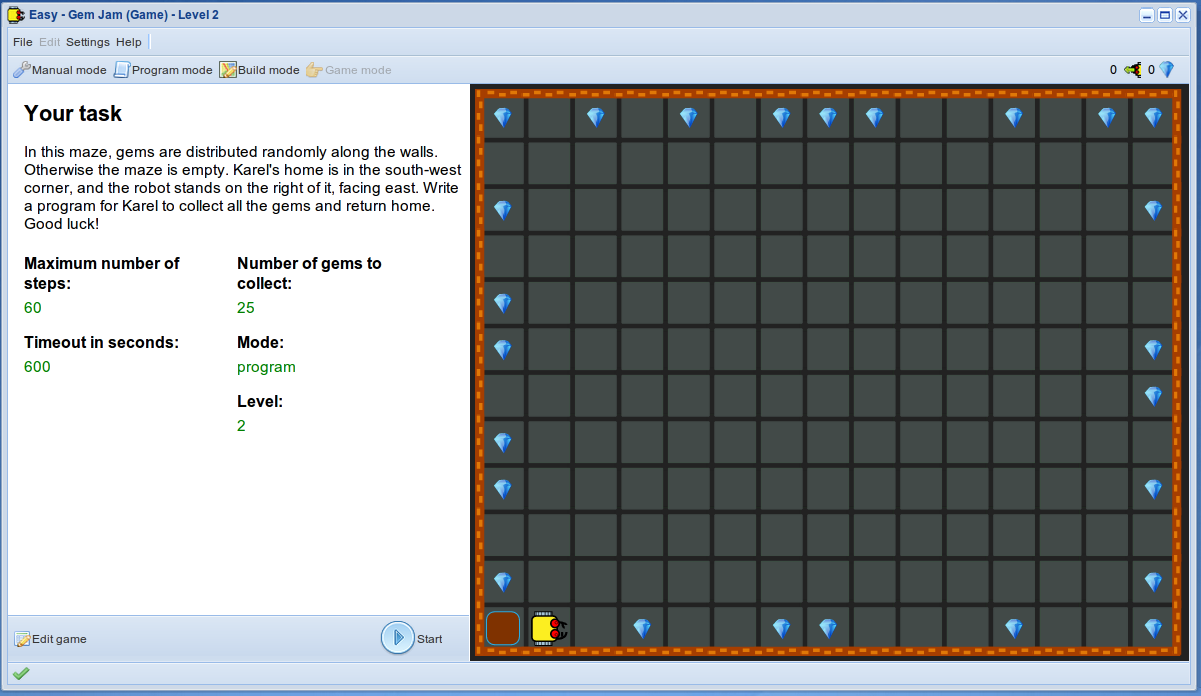
\includegraphics[width=0.7\textwidth]{img/g05.png}
\end{center}
\vspace{-4mm}
\caption{Gem Jam!}
\label{fig:g05}
\vspace{-10mm}
\end{figure}
\noindent

\newpage

\subsection{\ \ Exercise F11 - The Matrix}

{\em Write a program for Karel to collect all gems and get back home! The record is 
210 steps made. Can you do it with fewer steps?}

\begin{figure}[!ht]
\begin{center}
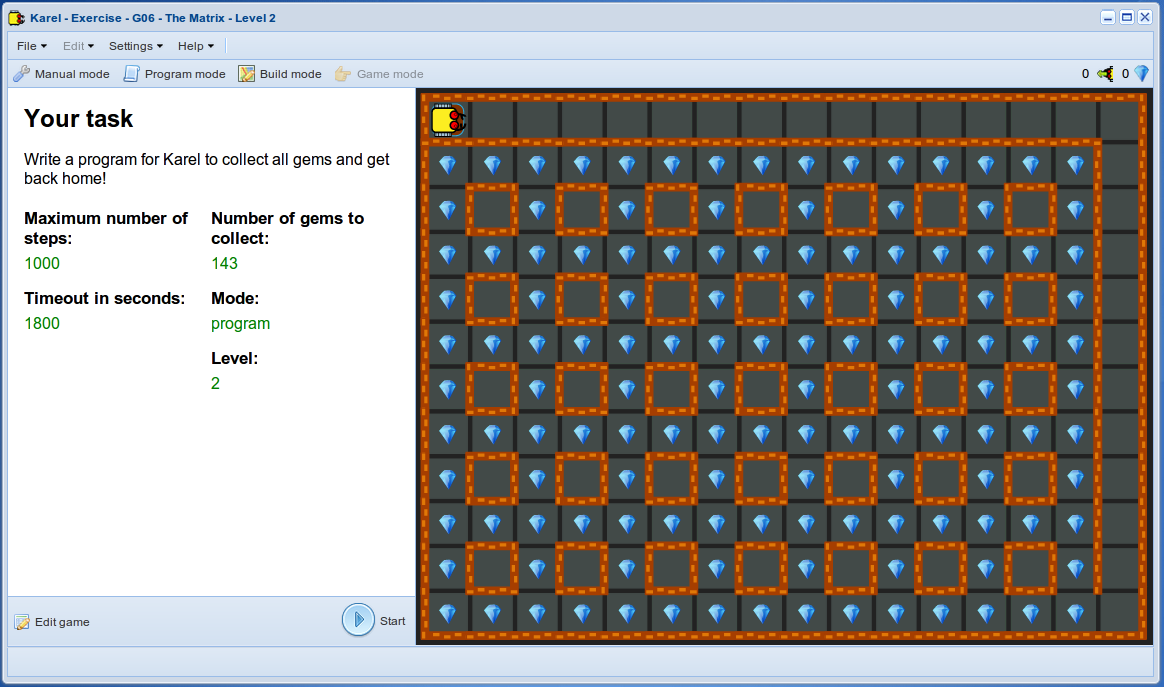
\includegraphics[width=0.7\textwidth]{img/g06.png}
\end{center}
\vspace{-4mm}
\caption{The Matrix.}
\label{fig:g06}
\vspace{-10mm}
\end{figure}
\noindent

\subsection{\ \ Exercise F12 - Escape from Alcatraz}

{\em Karel is escaping from the Alcatraz prison! At the moment he is in an underground labyrinth with many tunnels but only one of them leads to his freedom. He cannot know which one is it, so he needs to search them one by one. Start by going straight ahead to the nearest wall. Then use the right-hand rule to search the tunnels.}

\newpage

\begin{figure}[!ht]
\begin{center}
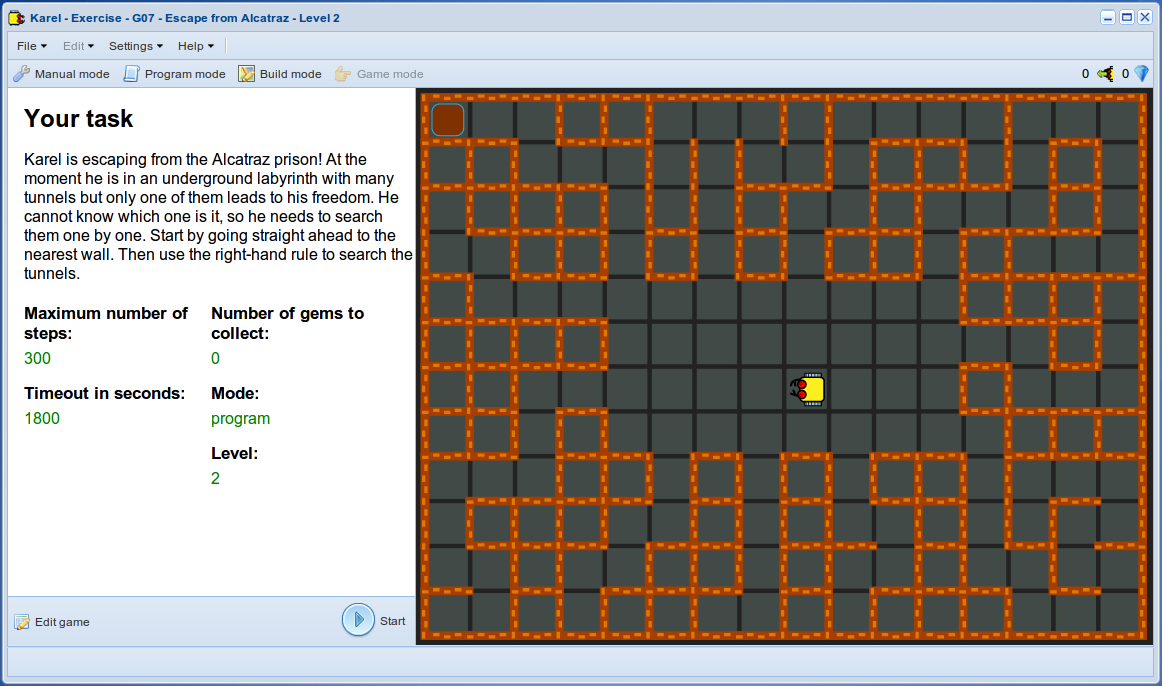
\includegraphics[width=0.7\textwidth]{img/g07.png}
\end{center}
\vspace{-4mm}
\caption{Karel is escaping from the Alcatraz prison.}
\label{fig:g07}
\vspace{-8mm}
\end{figure}
\noindent

\subsection{\ \ Exercise F13 - Border Patrol}

{\em Write a program for Karel to check the perimeter of the maze using the 
right-hand rule. Do not forget to pick up all gems that you find on the way.}

\begin{figure}[!ht]
\begin{center}
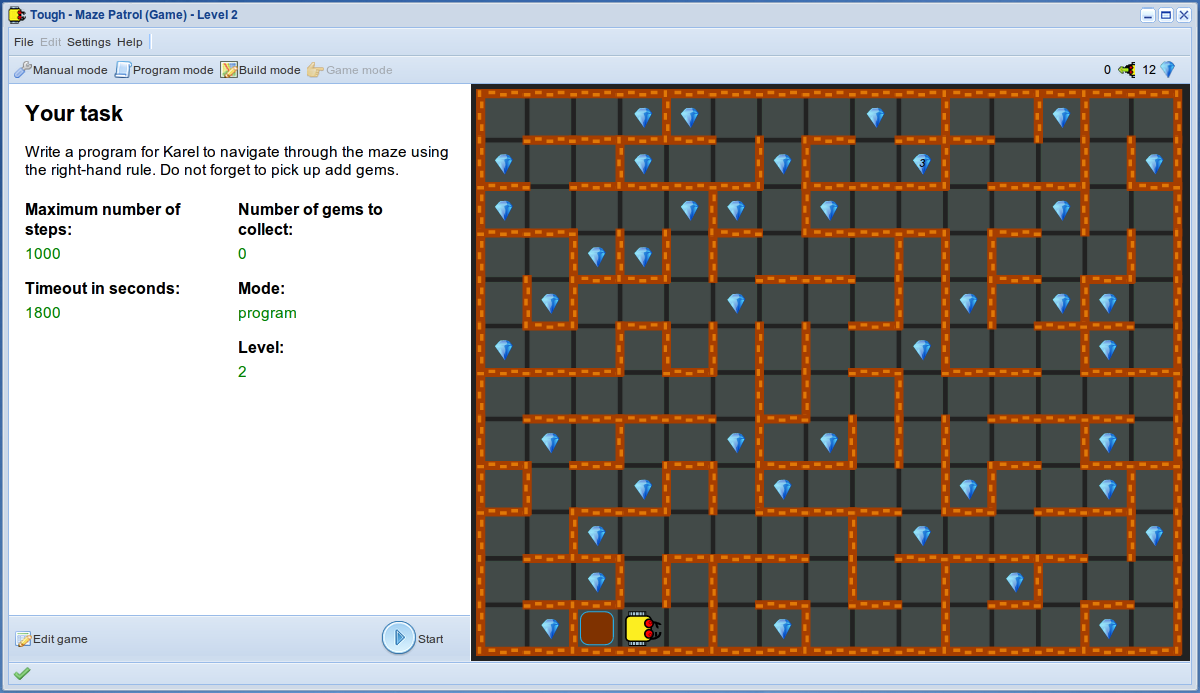
\includegraphics[width=0.7\textwidth]{img/g08.png}
\end{center}
\vspace{-4mm}
\caption{Border Patrol.}
\label{fig:g08}
\vspace{-10mm}
\end{figure}
\noindent

\subsection{\ \ Exercise F14 - Ariadne's Thread}

{\em In an ancient Greek legend, princess Ariadne saved the life of her 
beloved Theseus by giving him a thread that he used to avoid getting lost 
in the maze of king Minos and kill a feared beast Minotaurus. Karel uses 
a similar technique - he leaves behind him a chain of gems that helps him 
to safely find his way back home. Your program needs to work for an 
arbitrary maze. You can assume that the string of gems is continuous 
and that it does not contain any loops.}

\begin{figure}[!ht]
\begin{center}
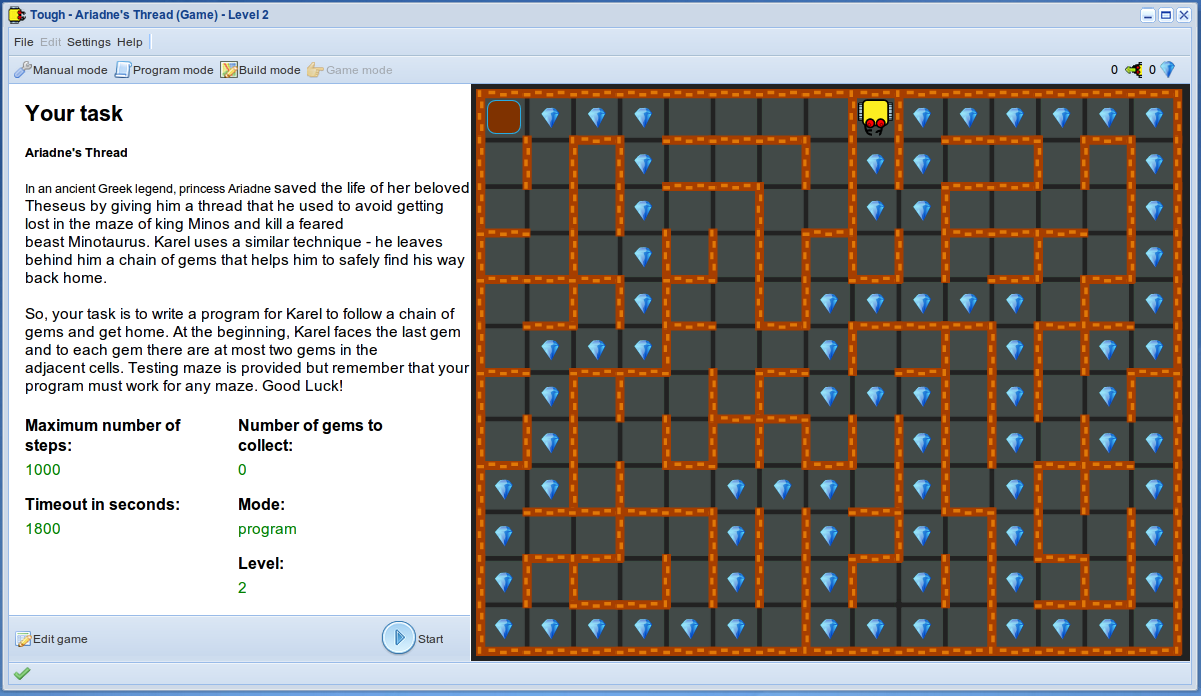
\includegraphics[width=0.7\textwidth]{img/g09.png}
\end{center}
\vspace{-4mm}
\caption{Maze of king Minos, home of the beast Minotaurus.}
\label{fig:g09}
\end{figure}
\noindent

\section{Section G - Logical Variables}

\subsection{Objectives} 
 
\begin{itemize}
\item Learn to work with elementary and complex logical operations.
\item Learn to define and use logical variables.
\end{itemize}

\noindent
In programming, variables are used to store information for later use. This information can 
be a number, word, sentence, or simply a "True" or "False". We will start
with the last type. 

\subsection{Simple logical expressions}
Logical expressions are expressions that can be answered with either "True" or 
"False". We say that the "True" or the "False" is their value. Here are some 
real-life examples, try to answer them with "True" or "False":

\begin{itemize}
\item "I am 15 years old."
\item "My dad is a teacher."
\item "My school's name is Coral Academy."
\end{itemize}
And here are some Karel examples:
\begin{itemize}
\item wall (True if the robot is facing a wall, False otherwise)
\item home (True if the robot is home, False otherwise)
\item gem (True if the robot stands on a gem, False otherwise)
\item north (True if the robot is facing North, False otherwise)
\item empty (True if the robot does not have any gems on him, False otherwise)
\end{itemize}

\subsection{Logical operations and logical variables}

In programming as well as in real life we often deal with logical expressions that are 
fairly complex. Often we use two or more simple logical expressions in one sentence, that 
are combined via logical operations.

For example, the sentence "I will go ski on Saturday if weather is good and if 
Michael goes as well." includes three simple logical expressions. Let's call 
them for brevity

\begin{itemize}
\item A = "I will go skiing on Saturday",
\item B = "the weather is good",
\item C = "Michael goes as well".  
\end{itemize}
There is also a logical operation "and" involved between the expressions B and C.

The original sentence can be written briefly as "if (B and C) then A". We love this kind of 
brevity in programming! The letters A, B and C are logical variables. Logical variables 
can only represent "True" or "False", and their purpose is to ease the operation with 
longer expressions.
Regarding the original sentence, we could go one step further and define a new logical variable\\

\noindent
D = B and C.\\

\noindent
Then, the sentence would become "if D then A". It is worth mentioning the following 
property of the logical "and":\\

\begin{center}
\framebox{(A and B) is True only if both A and B are True. Otherwise A and B is False.}
\end{center}
\vspace{4mm}
\noindent
We also have a logical "or" with the following property:\\

\begin{center}
\framebox{(A or B) is True if at least one of A, B is True. If both A. B are False, (A or B) is False.}
\end{center}
\vspace{4mm}
\noindent
We also use the logical operation "not" with the following property:\\

\begin{center}
\framebox{(not A) is True if A is False and vice versa.}
\end{center}


\subsection{Review questions}

\begin{enumerate}
\item What are {\em variables} used for in programming? 
\item What is a {\em logical expression}? 
\item A is True and B is False. What is then the value of (A and not (A or B)) ?
\item A is True and B is True. What is then the value of (A and not (A and not B)) ?
\end{enumerate}

\subsection{Exercise G01 - Numerology I}

{\em Each box contains an integer number between 0 and 9. The numbers are not known to Karel a-priori. He needs to enter each box and recognize the number in it. Let's call this number N. When he leaves the box, he needs to create a pile of N gems. The task finishes when this is done for all boxes and the robot gets home.}

\begin{figure}[!ht]
\begin{center}
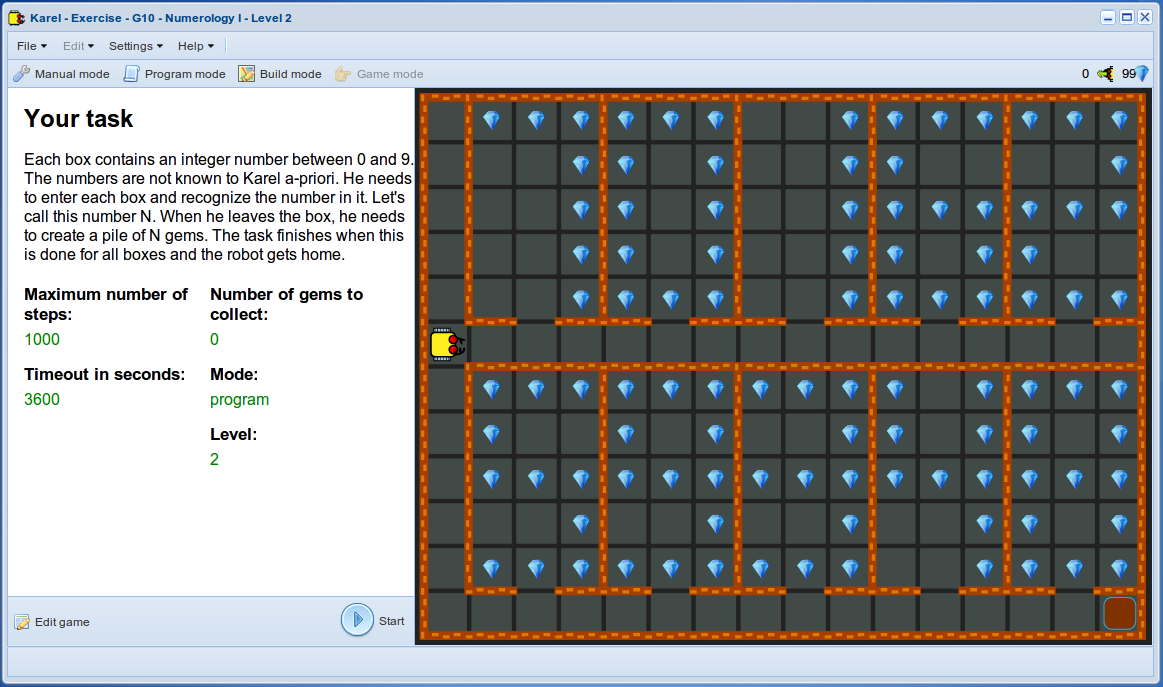
\includegraphics[width=0.7\textwidth]{img/g10.png}
\end{center}
\vspace{-4mm}
\caption{Karel decided to become a numerologist.}
\label{fig:g10}
\vspace{-4mm}
\end{figure}
\noindent

\subsection{Exercise G02 - Numerology II}

{\em There is a pile of N gems before the entrance to the box. It is known that N is between zero and 9. Karel needs to enter the box and render the number N. The task finishes when this is done and the robot gets home.}

\newpage
\begin{figure}[!ht]
\begin{center}
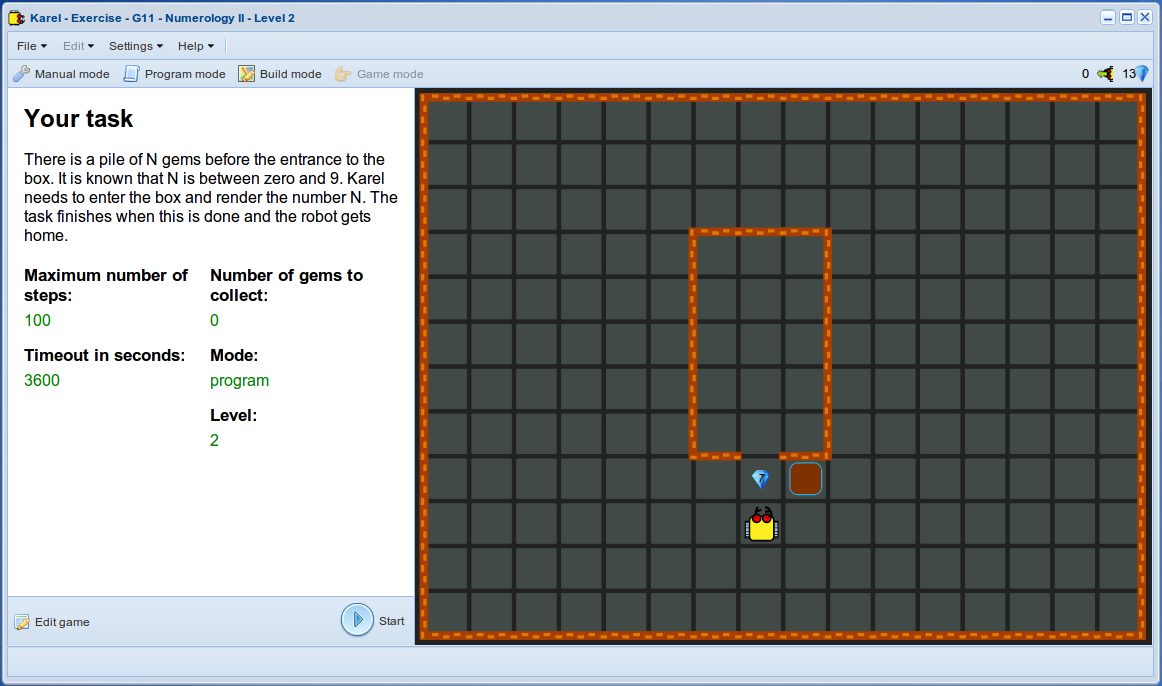
\includegraphics[width=0.7\textwidth]{img/g11.png}
\end{center}
\vspace{-4mm}
\caption{Karel is typing numbers.}
\label{fig:g11}
\vspace{-4mm}
\end{figure}
\noindent

\subsection{Exercise G03 - Numerology III}

{\em Add the numbers! Remember - Karel cannot see what numbers are in the boxes as you can see them. They can be any integers between 0 and 9. The task finishes when the robot gets home.}


\begin{figure}[!ht]
\begin{center}
\includegraphics[width=0.7\textwidth]{img/g12.png}
\end{center}
\vspace{-4mm}
\caption{Adding numbers without using math!}
\label{fig:g12}
\vspace{-4mm}
\end{figure}
\noindent

\subsection{Exercise G04 - Eight Queens}

{\em Karel stands on an 8 x 8 chess board along with eight queens (the gems). Recall that a chess queen dominates its row, its column, as well as both diagonals that pass through her position. Nothing may stand in these fields or she will destroy it. Currently, some queens are threatening each other. Write a program for Karel to correct the positions of the queens in such a way that none of them is threatened. Your program should be able to do it for any initial distribution of the queens. Enter the home after you are finished.}

\begin{figure}[!ht]
\begin{center}
\includegraphics[width=0.7\textwidth]{img/g14.png}
\end{center}
\vspace{-4mm}
\caption{The famous eight queens problem.}
\label{fig:g14}
\vspace{-4mm}
\end{figure}
\noindent

\subsection{Exercise G05 - BubbleSort}

{\em Karel stands in front of four piles of gems, let's enumerate them by 1, 2, 3 and 4. He does not know how many gems are in each pile. All he knows is that each pile contains between 1 and 4 gems, and that two or more piles can be equally large. Sort the piles in such a way that the smallest pile is on the left and the largest on the right. Use the BubbleSort algorithm: Implement a function that switches two adjacent piles if the one on the right has fewer gems than the one on the left. Apply this function to piles 1 and 2, then to piles 2 and 3, then to piles 3 and 4. Now it is certain that the largest number is on the right-most position! Next, do the same for just the first three piles. Last, apply the function to piles 1 and 2, and you are done! }

\newpage 

\begin{figure}[!ht]
\begin{center}
\includegraphics[width=0.7\textwidth]{img/g13.png}
\end{center}
\vspace{-4mm}
\caption{Karel is sorting four piles of gems.}
\label{fig:g13}
\vspace{-4mm}
\end{figure}
\noindent








\section{What Next?}

Congratulations on making it to the end of the tutorial! We hope that you
enjoyed it. If you can think of any ways to improve the application 
Karel the Robot in NCLab or this tutorial, please let us know. If you 
have an interesting game for Karel, please let us know as well. 

Although you may feel like an Almighty Programmer right now, we would
recommend staying humble. Even the most experienced programmers are
learning new things all the time. If you enjoy programming, your next 
language to learn may be Python. We have a Python Programming tutorial
in NCLab for you. We would also recommend that you learn Javascript since this 
is the most popular language for web development. Depending on your 
other hobbies or interests, C++ or even Fortran might be interesting. 
In any case, the NCLab Team wishes you good luck, and keep us in your 
favorite bookmarks!\\
\\
\hbox{} \hfill Your NCLab Team






\end{document}
